%
% ---------------------------------------------------------------
% Copyright (C) 2012-2018 Gang Li
% ---------------------------------------------------------------
%
% This work is the default powerdot-tuliplab style test file and may be
% distributed and/or modified under the conditions of the LaTeX Project Public
% License, either version 1.3 of this license or (at your option) any later
% version. The latest version of this license is in
% http://www.latex-project.org/lppl.txt and version 1.3 or later is part of all
% distributions of LaTeX version 2003/12/01 or later.
%
% This work has the LPPL maintenance status "maintained".
%
% This Current Maintainer of this work is Gang Li.
%
%

\documentclass[
 size=14pt,
 paper=smartboard,  %a4paper, smartboard, screen
 mode=present, 		%present, handout, print
 display=slides, 	% slidesnotes, notes, slides
 style=tuliplab,  	% TULIP Lab style
 pauseslide,
 fleqn,leqno]{powerdot}


\usepackage{cancel}
\usepackage{caption}
\usepackage{stackengine}
\usepackage{smartdiagram}
\usepackage{attrib}
\usepackage{amssymb}
\usepackage{amsmath} 
\usepackage{amsthm} 
\usepackage{mathtools}
\usepackage{rotating}
\usepackage{graphicx}
\usepackage{boxedminipage}
\usepackage{rotate}
\usepackage{calc}
\usepackage[absolute]{textpos}
\usepackage{psfrag,overpic}
\usepackage{fouriernc}
\usepackage{pstricks,pst-3d,pst-grad,pstricks-add,pst-text,pst-node,pst-tree}
\usepackage{moreverb,epsfig,subfigure}
\usepackage{color}
\usepackage{booktabs}
\usepackage{etex}
\usepackage{breqn}
\usepackage{multirow}
\usepackage{natbib}
\usepackage{bibentry}
\usepackage{gitinfo2}
\usepackage{siunitx}
\usepackage{nicefrac}
%\usepackage{geometry}
%\geometry{verbose,letterpaper}
\usepackage{media9}
\usepackage{animate}
%\usepackage{movie15}
\usepackage{auto-pst-pdf}

\usepackage{breakurl}
\usepackage{fontawesome}
\usepackage{xcolor}
\usepackage{multicol}



\usepackage{verbatim}
\usepackage[utf8]{inputenc}
\usepackage{dtk-logos}
\usepackage{tikz}
\usepackage{adigraph}
%\usepackage{tkz-graph}
\usepackage{hyperref}
%\usepackage{ulem}
\usepackage{pgfplots}
\usepackage{verbatim}
\usepackage{fontawesome}


\usepackage{todonotes}
% \usepackage{pst-rel-points}
\usepackage{animate}
\usepackage{fontawesome}

\usepackage{listings}
\lstset{frameround=fttt,
frame=trBL,
stringstyle=\ttfamily,
backgroundcolor=\color{yellow!20},
basicstyle=\footnotesize\ttfamily}
\lstnewenvironment{code}{
\lstset{frame=single,escapeinside=`',
backgroundcolor=\color{yellow!20},
basicstyle=\footnotesize\ttfamily}
}{}


\usepackage{hyperref}
\hypersetup{ % TODO: PDF meta Data
  pdftitle={Presentation Title},
  pdfauthor={Gang Li},
  pdfpagemode={FullScreen},
  pdfborder={0 0 0}
}


% \usepackage{auto-pst-pdf}
% package to show source code

\definecolor{LightGray}{rgb}{0.9,0.9,0.9}
\newlength{\pixel}\setlength\pixel{0.000714285714\slidewidth}
\setlength{\TPHorizModule}{\slidewidth}
\setlength{\TPVertModule}{\slideheight}
\newcommand\highlight[1]{\fbox{#1}}
\newcommand\icite[1]{{\footnotesize [#1]}}

\newcommand\twotonebox[2]{\fcolorbox{pdcolor2}{pdcolor2}
{#1\vphantom{#2}}\fcolorbox{pdcolor2}{white}{#2\vphantom{#1}}}
\newcommand\twotoneboxo[2]{\fcolorbox{pdcolor2}{pdcolor2}
{#1}\fcolorbox{pdcolor2}{white}{#2}}
\newcommand\vpspace[1]{\vphantom{\vspace{#1}}}
\newcommand\hpspace[1]{\hphantom{\hspace{#1}}}
\newcommand\COMMENT[1]{}

\newcommand\placepos[3]{\hbox to\z@{\kern#1
        \raisebox{-#2}[\z@][\z@]{#3}\hss}\ignorespaces}

\renewcommand{\baselinestretch}{1.2}


\newcommand{\draftnote}[3]{
	\todo[author=#2,color=#1!30,size=\footnotesize]{\textsf{#3}}	}
% TODO: add yourself here:
%
\newcommand{\gangli}[1]{\draftnote{blue}{GLi:}{#1}}
\newcommand{\shaoni}[1]{\draftnote{green}{sn:}{#1}}
\newcommand{\gliMarker}
	{\todo[author=GLi,size=\tiny,inline,color=blue!40]
	{Gang Li has worked up to here.}}
\newcommand{\snMarker}
	{\todo[author=Sn,size=\tiny,inline,color=green!40]
	{Shaoni has worked up to here.}}

%%%%%%%%%%%%%%%%%%%%%%%%%%%%%%%%%%%%%%%%%%%%%%%%%%%%%%%%%%%%%%%%%%%%%%%%
% title
% TODO: Customize to your Own Title, Name, Address
%
\title{Titanic Survial Prediction}
\author{
Pratikshya Parajuli
\\
\\Ministry of Finance
\\Governmnet of Nepal
\\
}
%\date{\gitCommitterDate}


% Customize the setting of slides
\pdsetup{
% TODO: Customize the left footer, and right footer
rf=\href{http://www.tulip.org.au}{
Last Changed by: \textsc{\gitCommitterName}\ \gitVtagn-\gitAbbrevHash\ (\gitAuthorDate)
},
cf={Titanic Survial Prediction},
}


\begin{document}

\maketitle

\begin{slide}{Overview}
\tableofcontents[content=sections]
\end{slide}


%%==========================================================================================

%%==========================================================================================


\section{Introduction}


%%==========================================================================================
%%
\begin{slide}{Overview}
\begin{center}
\twotonebox{\rotatebox{90}{}}{\parbox{.86\textwidth}
{The sinking of the Titanic is one of the most infamous shipwrecks in history. This project aims to create a model that predicts which passengers survived the disaster.
\begin{itemize}
\item Useful features are \textcolor{orange}{Pclass, Name, Sex, Age, SibSp, Parch, Ticket, Fare, Cabin, Embarked} 
\item Target feature is \textcolor{orange}{Survived}
\end{itemize}
}}

\end{center}
\bigskip
% \begin{figure}
%    \centering
%    \selectcolormodel{rgb}
%    \centerline{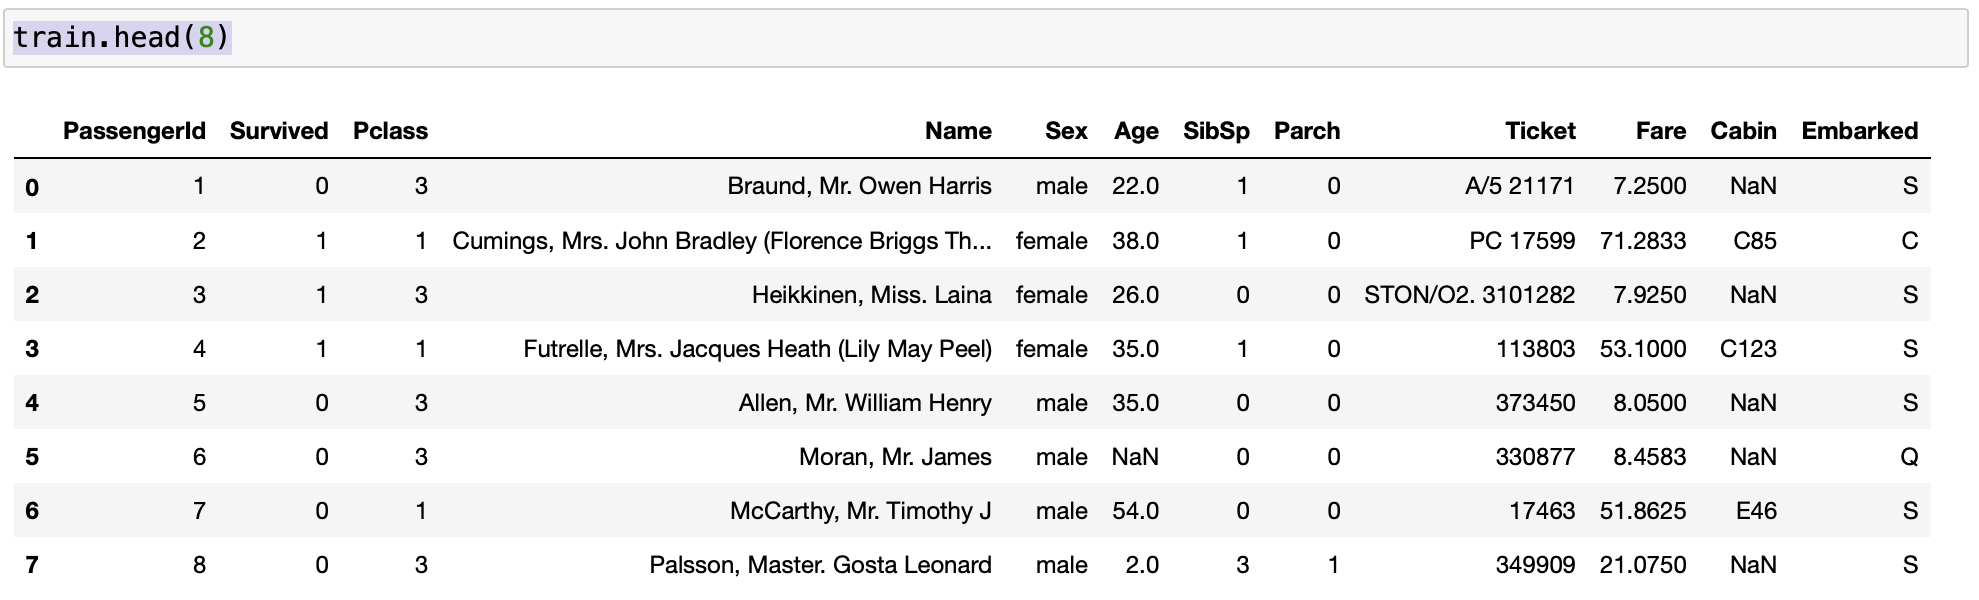
\includegraphics[width=1.5\textwidth,height=.5\textwidth]{/Users/pratikshyaparajuli/Desktop/kaggle/KaggleProject/Code/templatex/graphics/titanicimg/feature-data.png}}
%  \end{figure}
\bigskip
\end{slide}

%%
%%==========================================================================================
\section{Exploratory Data Analysis(EDA)}

\begin{slide}{Dataset}
  \twocolumn[
\savevalue{lfrheight}=4.6cm,
\savevalue{lfrprop}={
linestyle=solid,framearc=.2,linewidth=1pt},
rfrheight=\usevalue{lfrheight},
rfrprop=\usevalue{lfrprop}
]{
  \begin{figure}
    \centering
    %\selectcolormodel{rgb}
    \centerline{\includegraphics[width=1.0\textwidth,height=0.4\textwidth]{/Users/pratikshyaparajuli/Desktop/kaggle/KaggleProject/Code/templatex/graphics/titanicimg/datatable.eps}}
  \end{figure}
  }{
  \begin{figure}
    %\centering
    %\selectcolormodel{rgb}
    \centerline{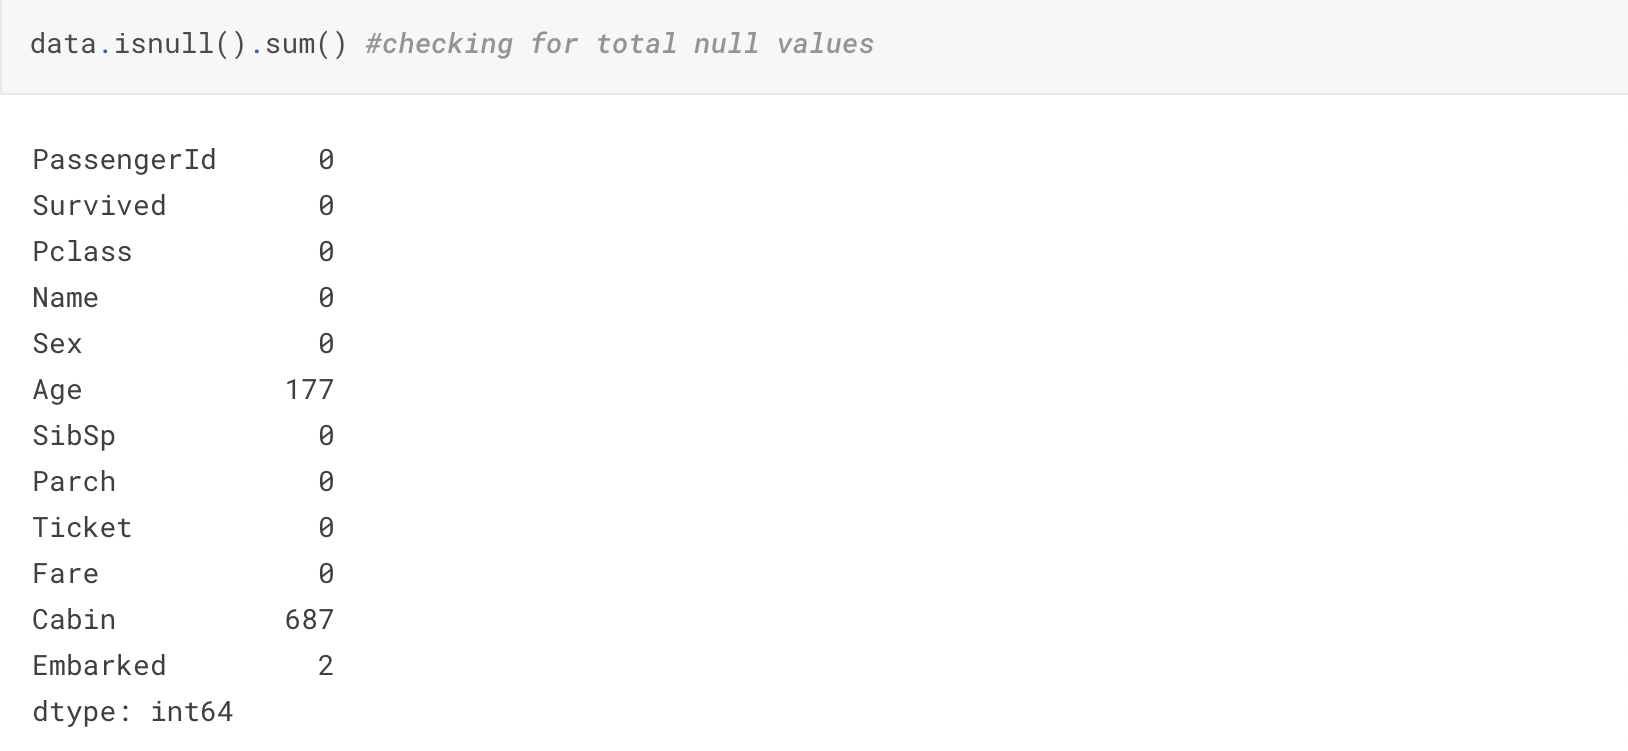
\includegraphics[width=1.0\textwidth,height=0.4\textwidth]{/Users/pratikshyaparajuli/Desktop/kaggle/KaggleProject/Code/templatex/graphics/titanicimg/null_values.eps}}
  \end{figure}
  }
  \begin{itemize}
    \item
    \textcolor{orange}{Age, Sex, Embarked} have null values.
    \end{itemize}
  \end{slide}
%%==========================================================================================
%%
\begin{slide}{How many Survived?}
 
  \begin{figure}
    \centering
    %\selectcolormodel{rgb}
    \centerline{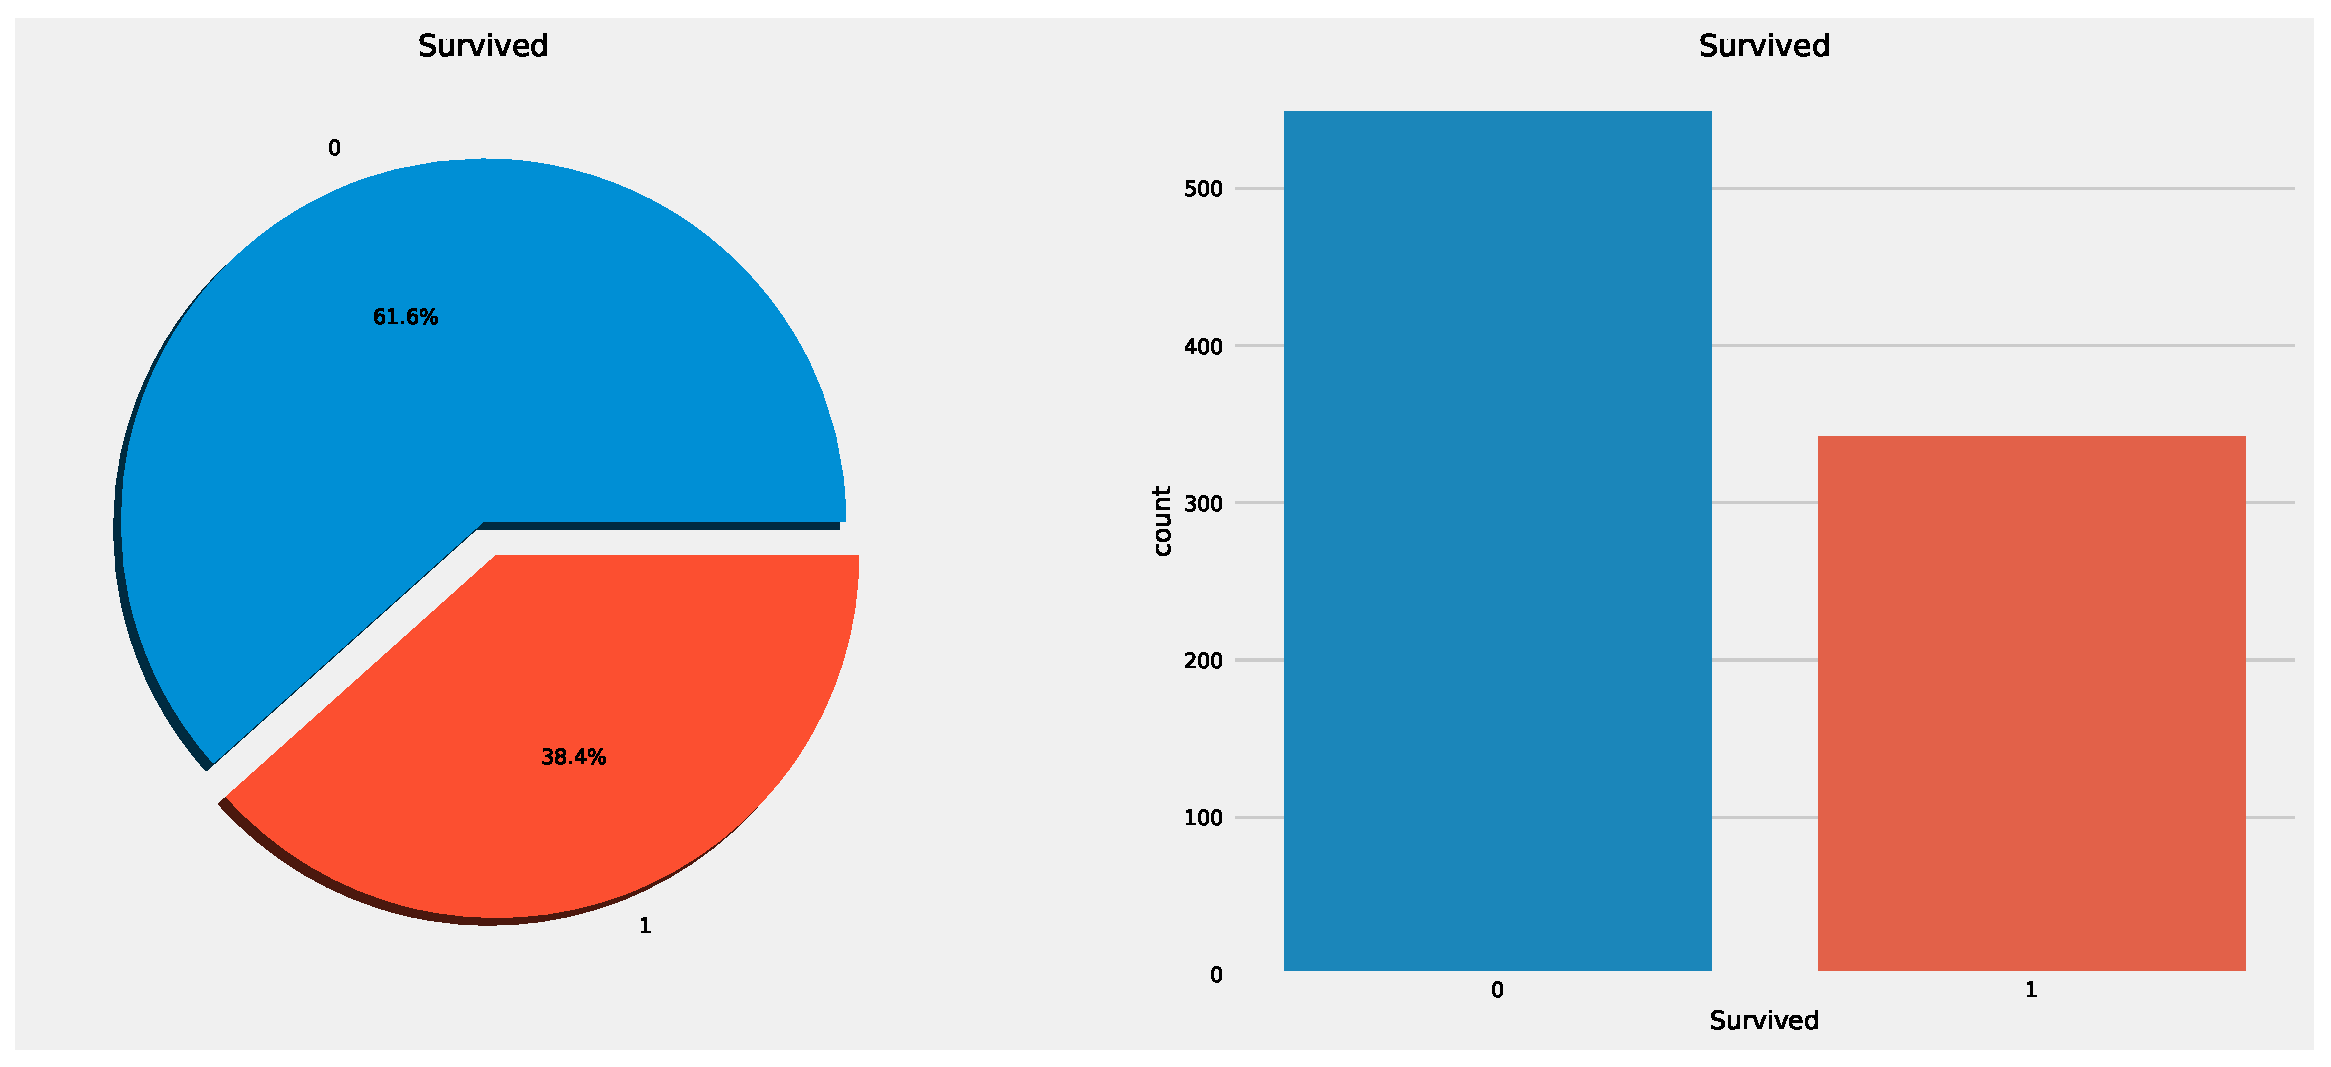
\includegraphics[width=1.0\textwidth,height=0.4\textwidth]{/Users/pratikshyaparajuli/Desktop/kaggle/KaggleProject/Code/templatex/graphics/titanicimg/Survived.eps}}
  \end{figure}
  \begin{itemize}
    \item
    We will try to check the survival rate by using the different features of the dataset. Some of the features being Sex, Port Of Embarcation, Age,etc.
    \end{itemize}
  \end{slide}
%%==========================================================================================
%%
\begin{slide}{Analysis of the Features}
\begin{itemize}
\item
Categorical Features in the dataset - \textcolor{orange}{Sex, Embarked}
\item
Ordinal Features in the dataset - \textcolor{orange}{Pclass}
\item
Continuous Features in the dataset - \textcolor{orange}{Age}
\end{itemize}
\begin{figure}
  \centering
  %\selectcolormodel{rgb}
  \centerline{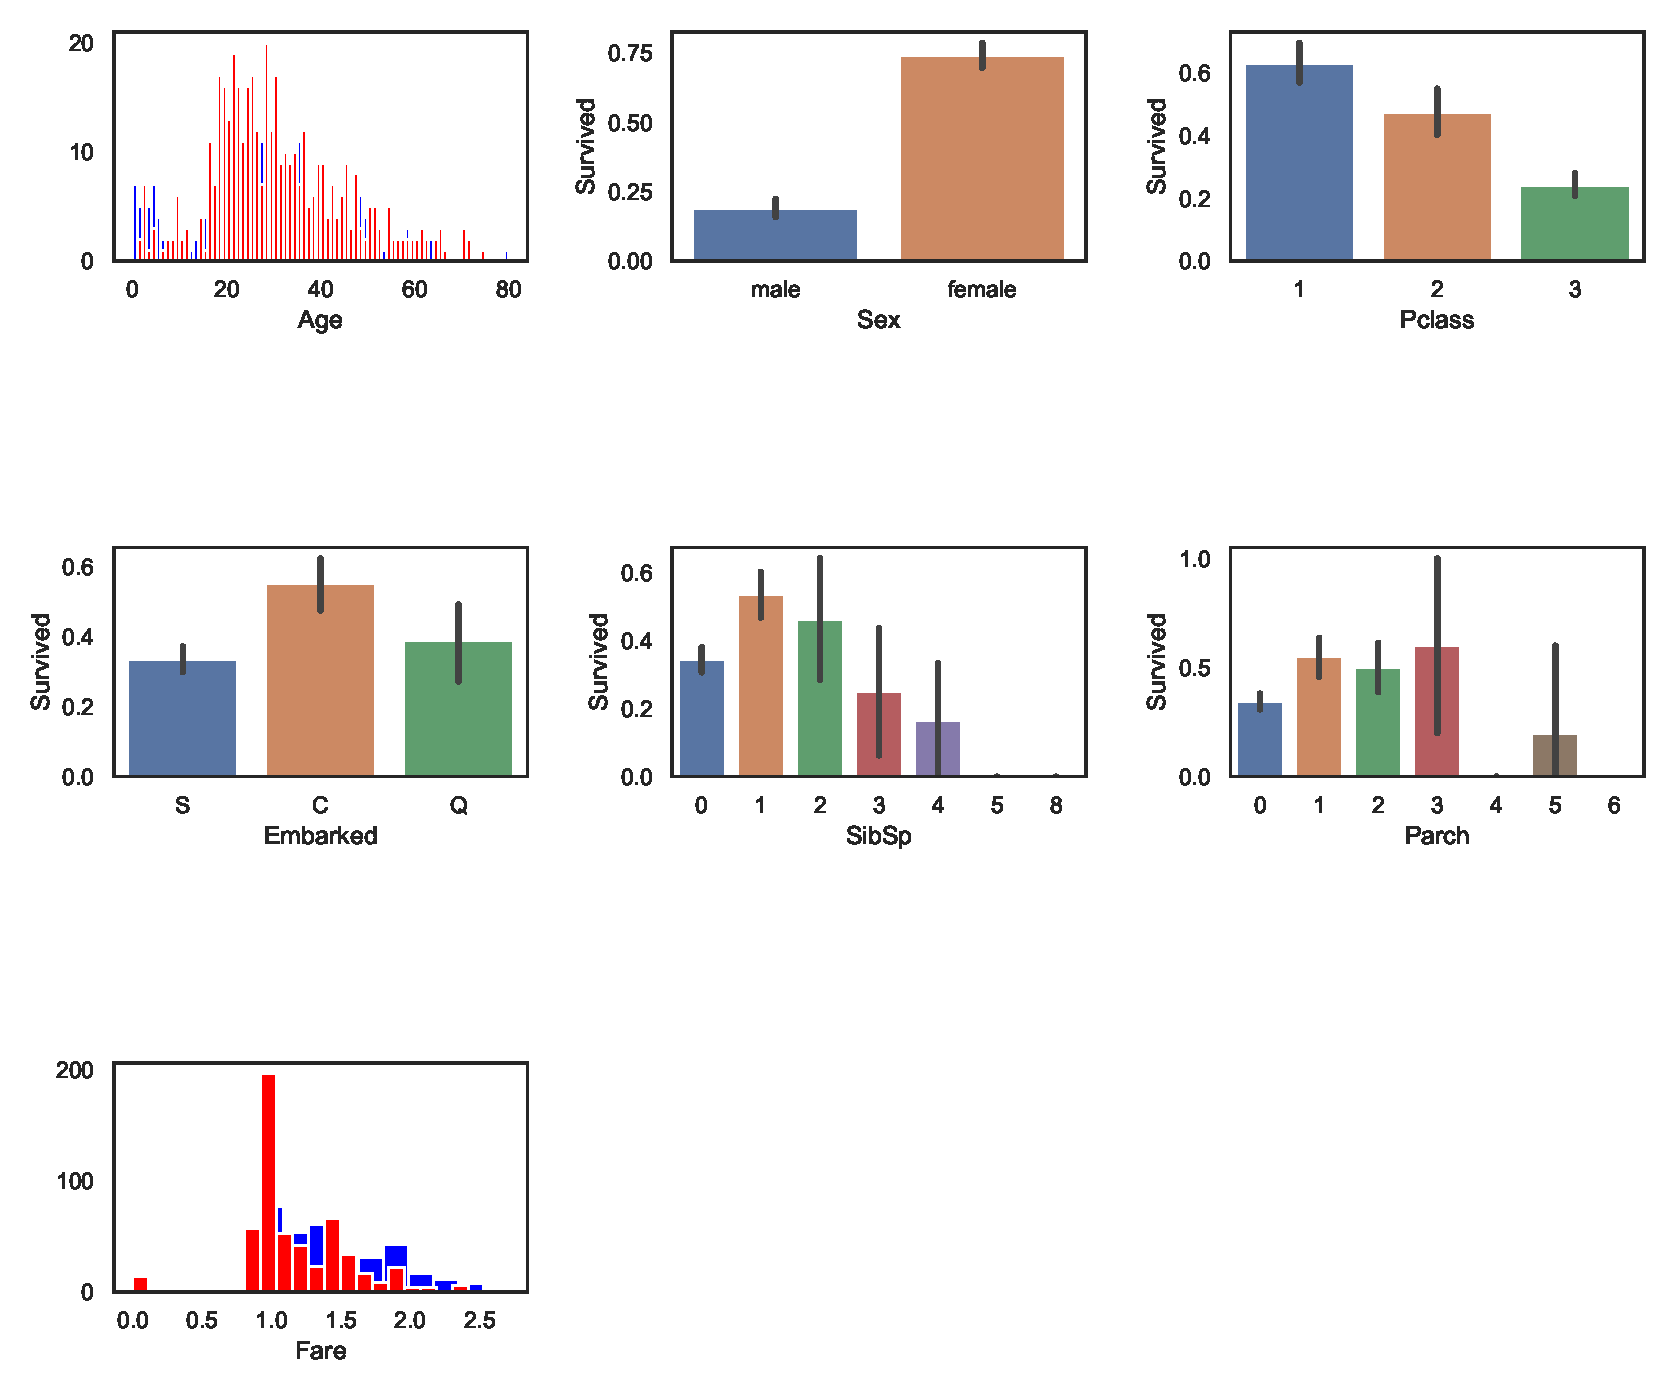
\includegraphics[width=1.0\textwidth,height=0.5\textwidth]{/Users/pratikshyaparajuli/Desktop/kaggle/KaggleProject/Code/templatex/graphics/titanicimg/allfeatures.eps}}
\end{figure}
\end{slide}
%%
%%
\begin{slide}[toc=,bm=]{Sex - Categorical Feature}
  \setlength{\abovecaptionskip}{0pt}
  \setlength{\belowcaptionskip}{10pt}
  \centering
  \begin{table}[tb]
    \setlength{\abovecaptionskip}{0pt}
    \setlength{\belowcaptionskip}{10pt}
    \centering
    \caption{Survived vs. Sex}
    
    \begin{tabular}{p{1.5cm}p{1.9cm}p{2.9cm}}
    \hline
      Sex & Survived & Numbers \\
    \hline
      Female   & 0    & 81 \\
        & 1 & 233 \\
      Male & 0  & 468 \\
        & 1  & 109  \\
    \hline
    \end{tabular}
    \end{table}
    \begin{figure}
      \centering
      %\selectcolormodel{rgb}
      \centerline{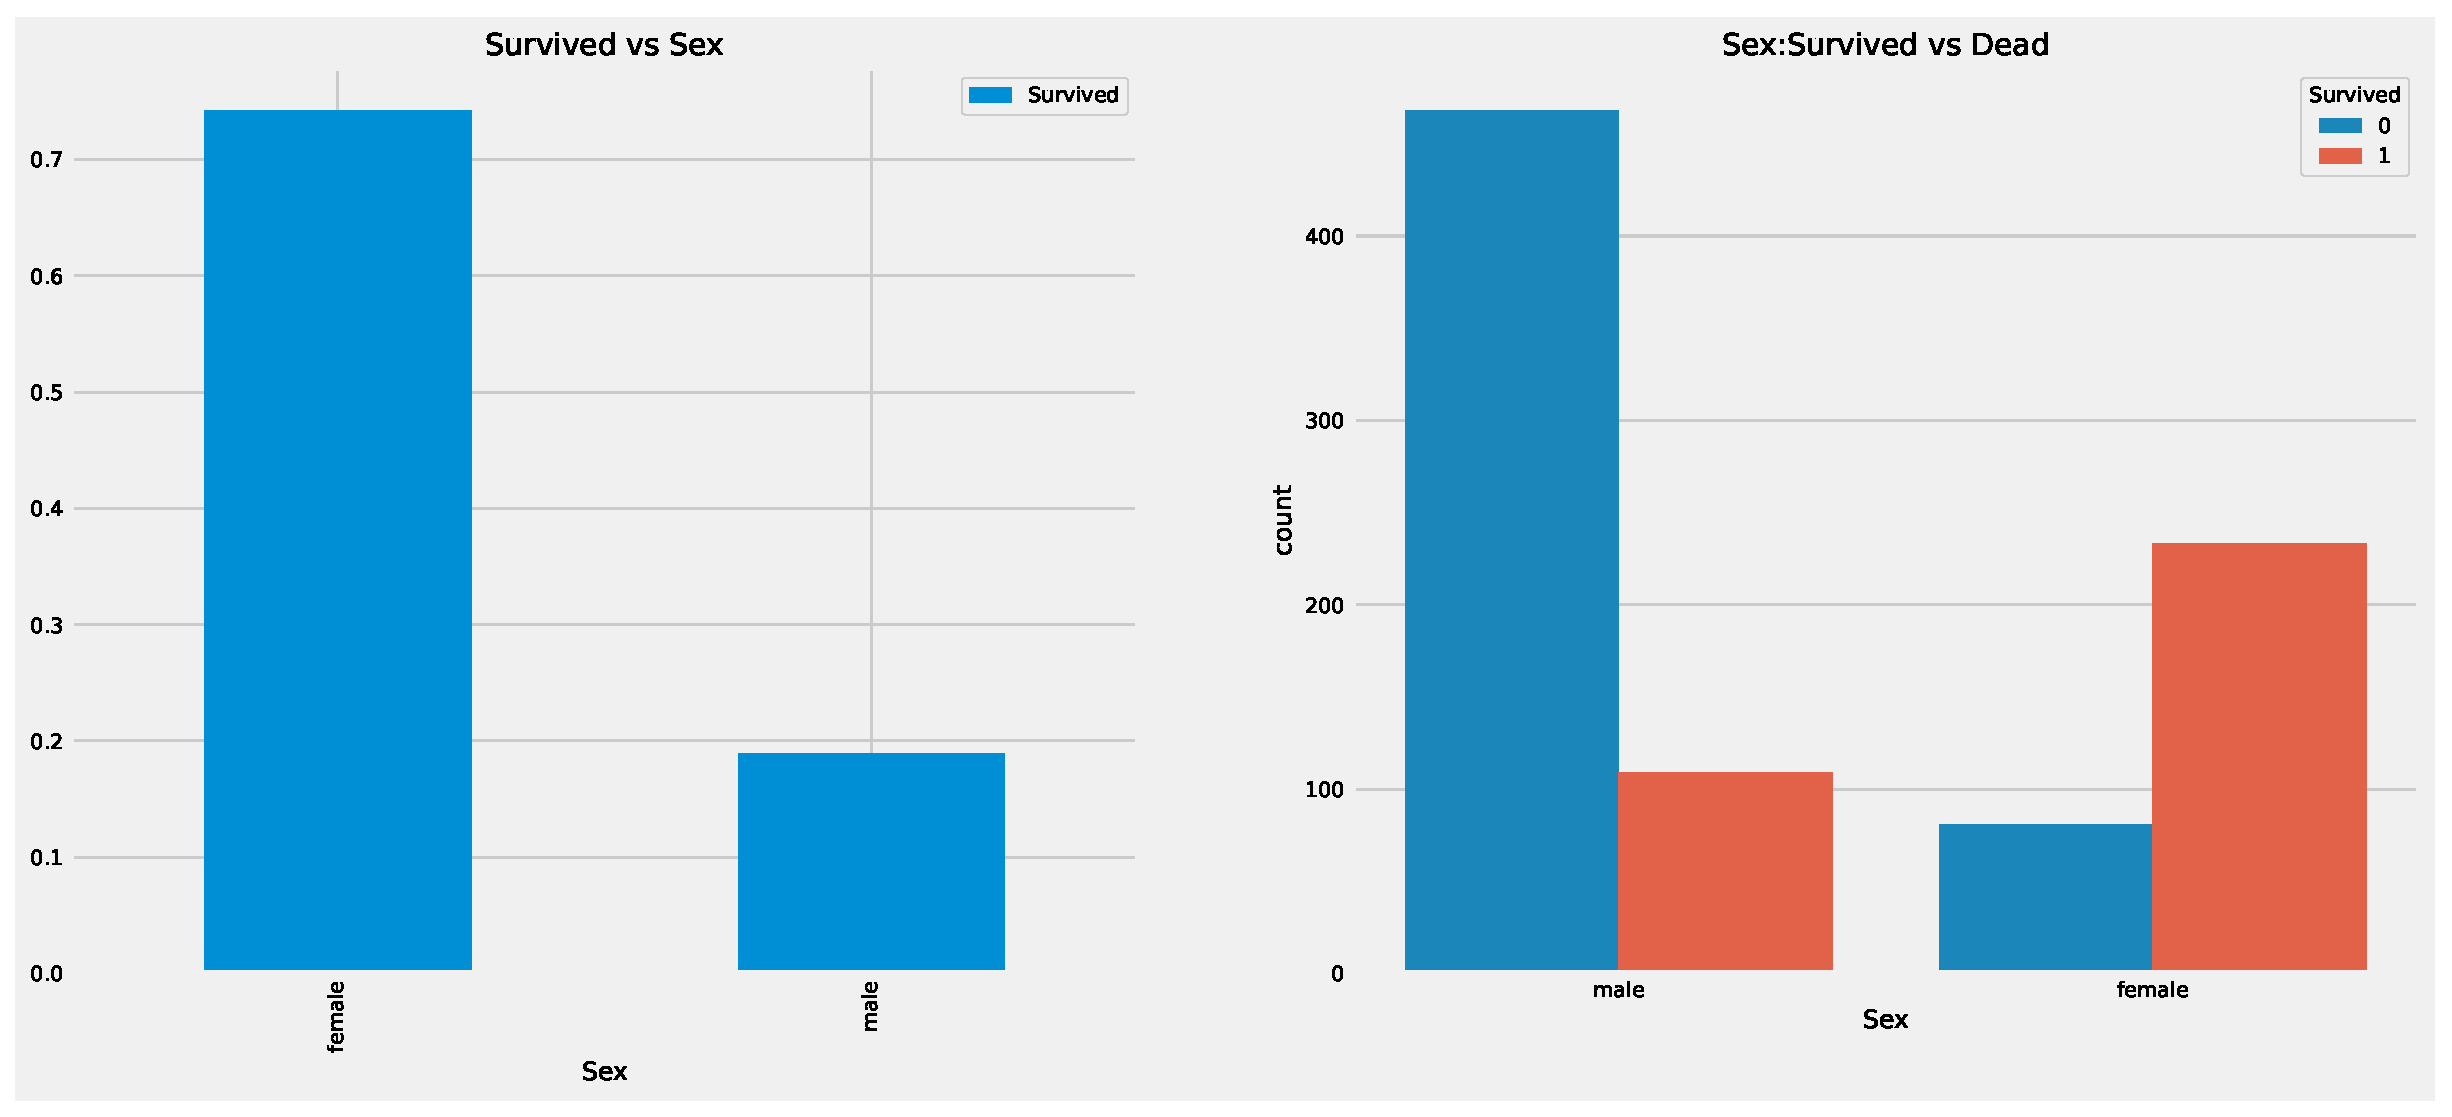
\includegraphics[width=0.5\textwidth,height=.2\textwidth]{/Users/pratikshyaparajuli/Desktop/kaggle/KaggleProject/Code/templatex/graphics/titanicimg/survivedvsdead.eps}}
    \end{figure}
    \begin{itemize}
      \item
      Survival rates for a women: \textcolor{orange}{75 percent and men: 18-19 percent}.
      \end{itemize}
\end{slide}
%%
%%
\begin{slide}[toc=,bm=]{Pclass - Ordianal Feature}
  \setlength{\abovecaptionskip}{0pt}
  \setlength{\belowcaptionskip}{10pt}
  \centering
  \begin{table}[tb]
    \setlength{\abovecaptionskip}{0pt}
    \setlength{\belowcaptionskip}{10pt}
    \centering
    \caption{Numbers of Passengers by Pclass}
    
    \begin{tabular}{p{1.5cm}p{1.9cm}p{2.9cm}p{2.9cm}}
    \hline
    Survived Pclass & 0 & 1 & All \\
    \hline
      1   & 80    & 136    &   216     \\
      2   & 97    & 87     &   184   \\
      3   & 372   & 119    &   491  \\
      All & 549   & 342    &   891 \\
    \hline
    \end{tabular}
    \end{table}
    \vspace{0.2cm}
%\vspace{0.1cm}
\begin{figure}
  \centering
  %\selectcolormodel{rgb}
  \centerline{
    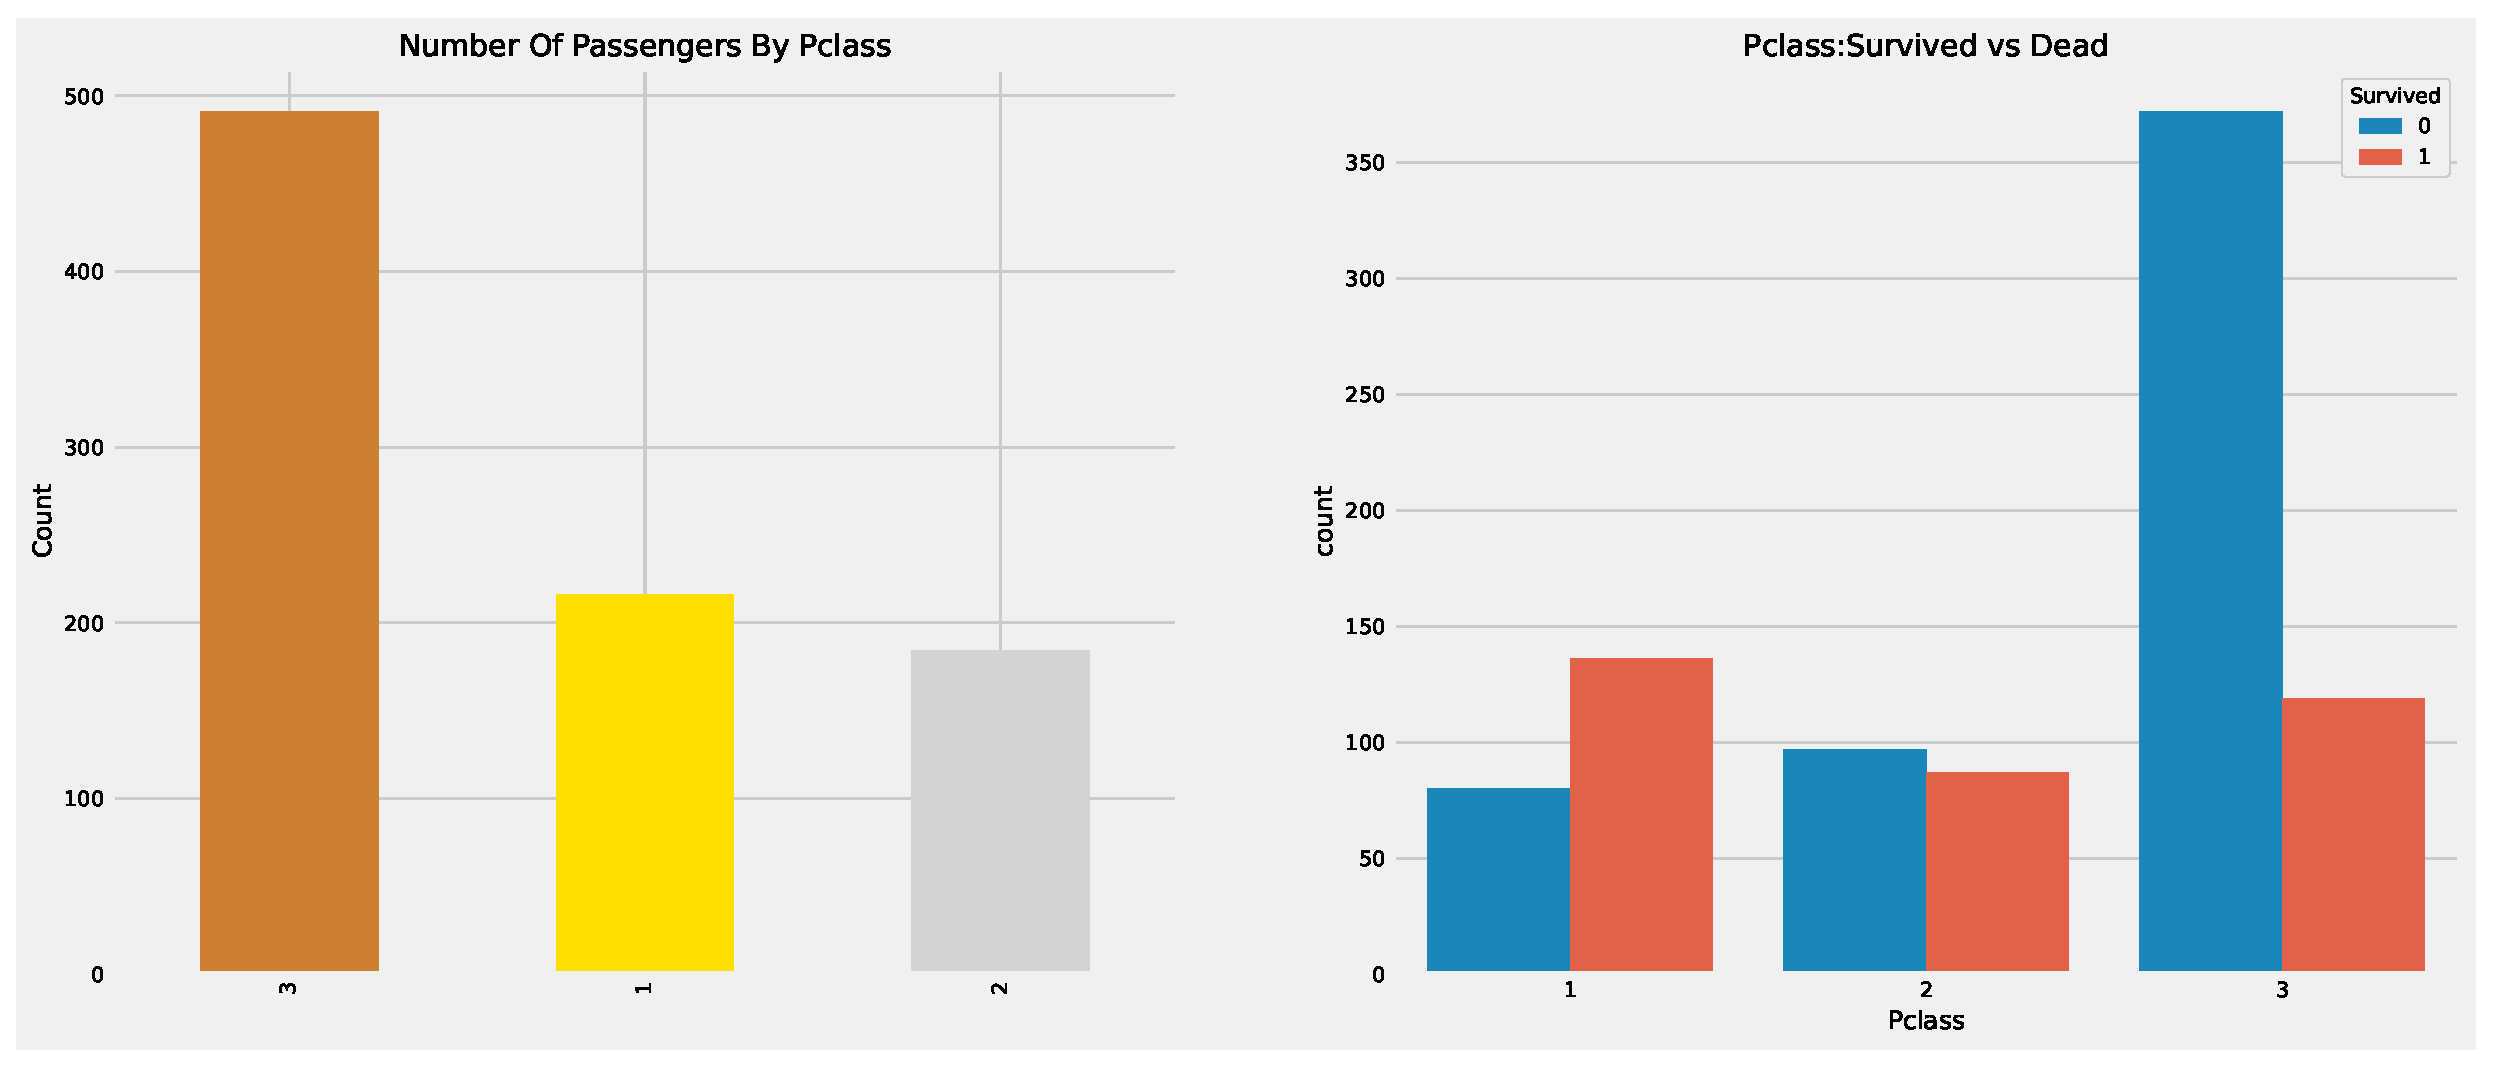
\includegraphics[width=0.5\textwidth,height=.2\textwidth]{/Users/pratikshyaparajuli/Desktop/kaggle/KaggleProject/Code/templatex/graphics/titanicimg/pclass.eps}
    }
    \caption{Pclass:Survived vs Dead}\label{fig:Pclass:Survived vs Dead}
\end{figure}
\end{slide}
%%
%%
\begin{slide}[toc=,bm=]{Survival rate with Sex and Pclass Together}
  \setlength{\abovecaptionskip}{0pt}
  \setlength{\belowcaptionskip}{10pt}
  \centering
  \begin{table}[tb]
    \setlength{\abovecaptionskip}{0pt}
    \setlength{\belowcaptionskip}{10pt}
    \centering
    \caption{Survival rate with Sex and Pclass Together}
    
    \begin{tabular}{p{1.5cm}p{1.9cm}p{1.5cm}p{1.9cm}p{2.9cm}p{2.9cm}}
    \hline
     Sex  & PclassSurvived & 1 & 2 &3  & All \\
    \hline
      Female  & 0    & 3    &  6    &  72   & 81  \\
              & 1    & 91   &  70   &  72   & 233  \\
      Male    & 0    & 77   &  91   &  300  & 468  \\
              & 1    & 45   &  17   &  47   & 109  \\
      All     &      & 216  &  184  &  491  & 891  \\
    \hline
    \end{tabular}
    \end{table}
    \vspace{0.1cm}
%\vspace{0.1cm}
\begin{figure}
  \centering
  %\selectcolormodel{rgb}
  %\missingfigure{Testing a long text string.}
  \centerline{
    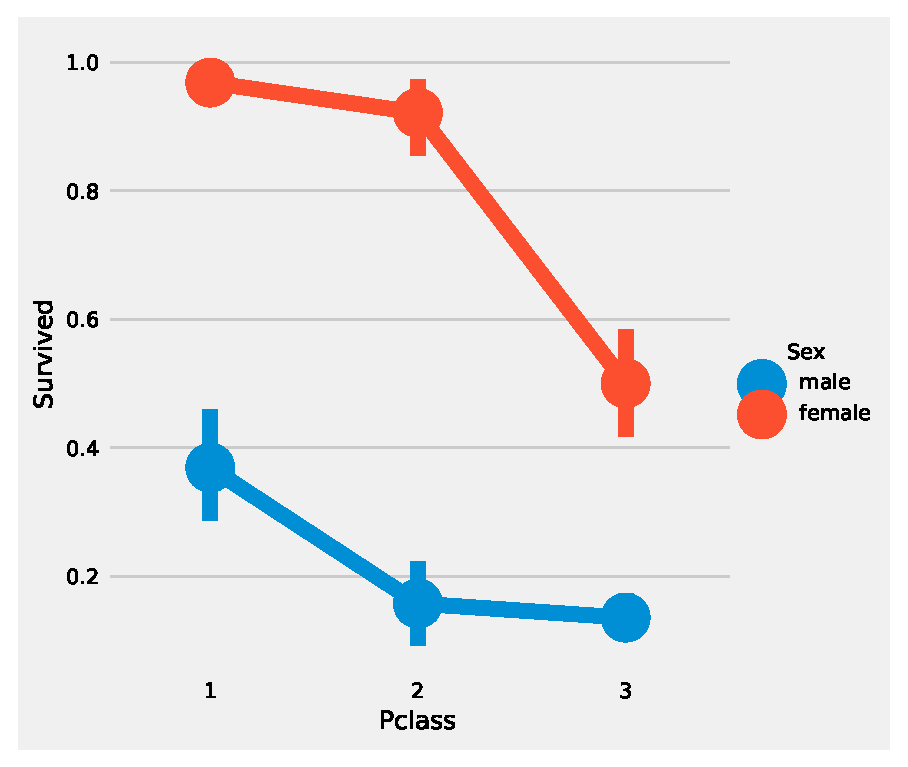
\includegraphics[width=0.5\textwidth,height=.2\textwidth]{/Users/pratikshyaparajuli/Desktop/kaggle/KaggleProject/Code/templatex/graphics/titanicimg/pclassvssex.eps}
    }
  \caption{Survival rate with Sex and Pclass Together}\label{fig:sexvspclass}
\end{figure}
\end{slide}
%%
%%
\begin{slide}[toc=,bm=]{Age - Continuous Feature}
  Oldest Passenger was of: 80.0 Years \\
  Youngest Passenger was of: 0.42 Years 
\vspace{0.1cm}
\begin{figure}
  \centering
  %\selectcolormodel{rgb}
  %\missingfigure{Testing a long text string.}
  \centerline{
    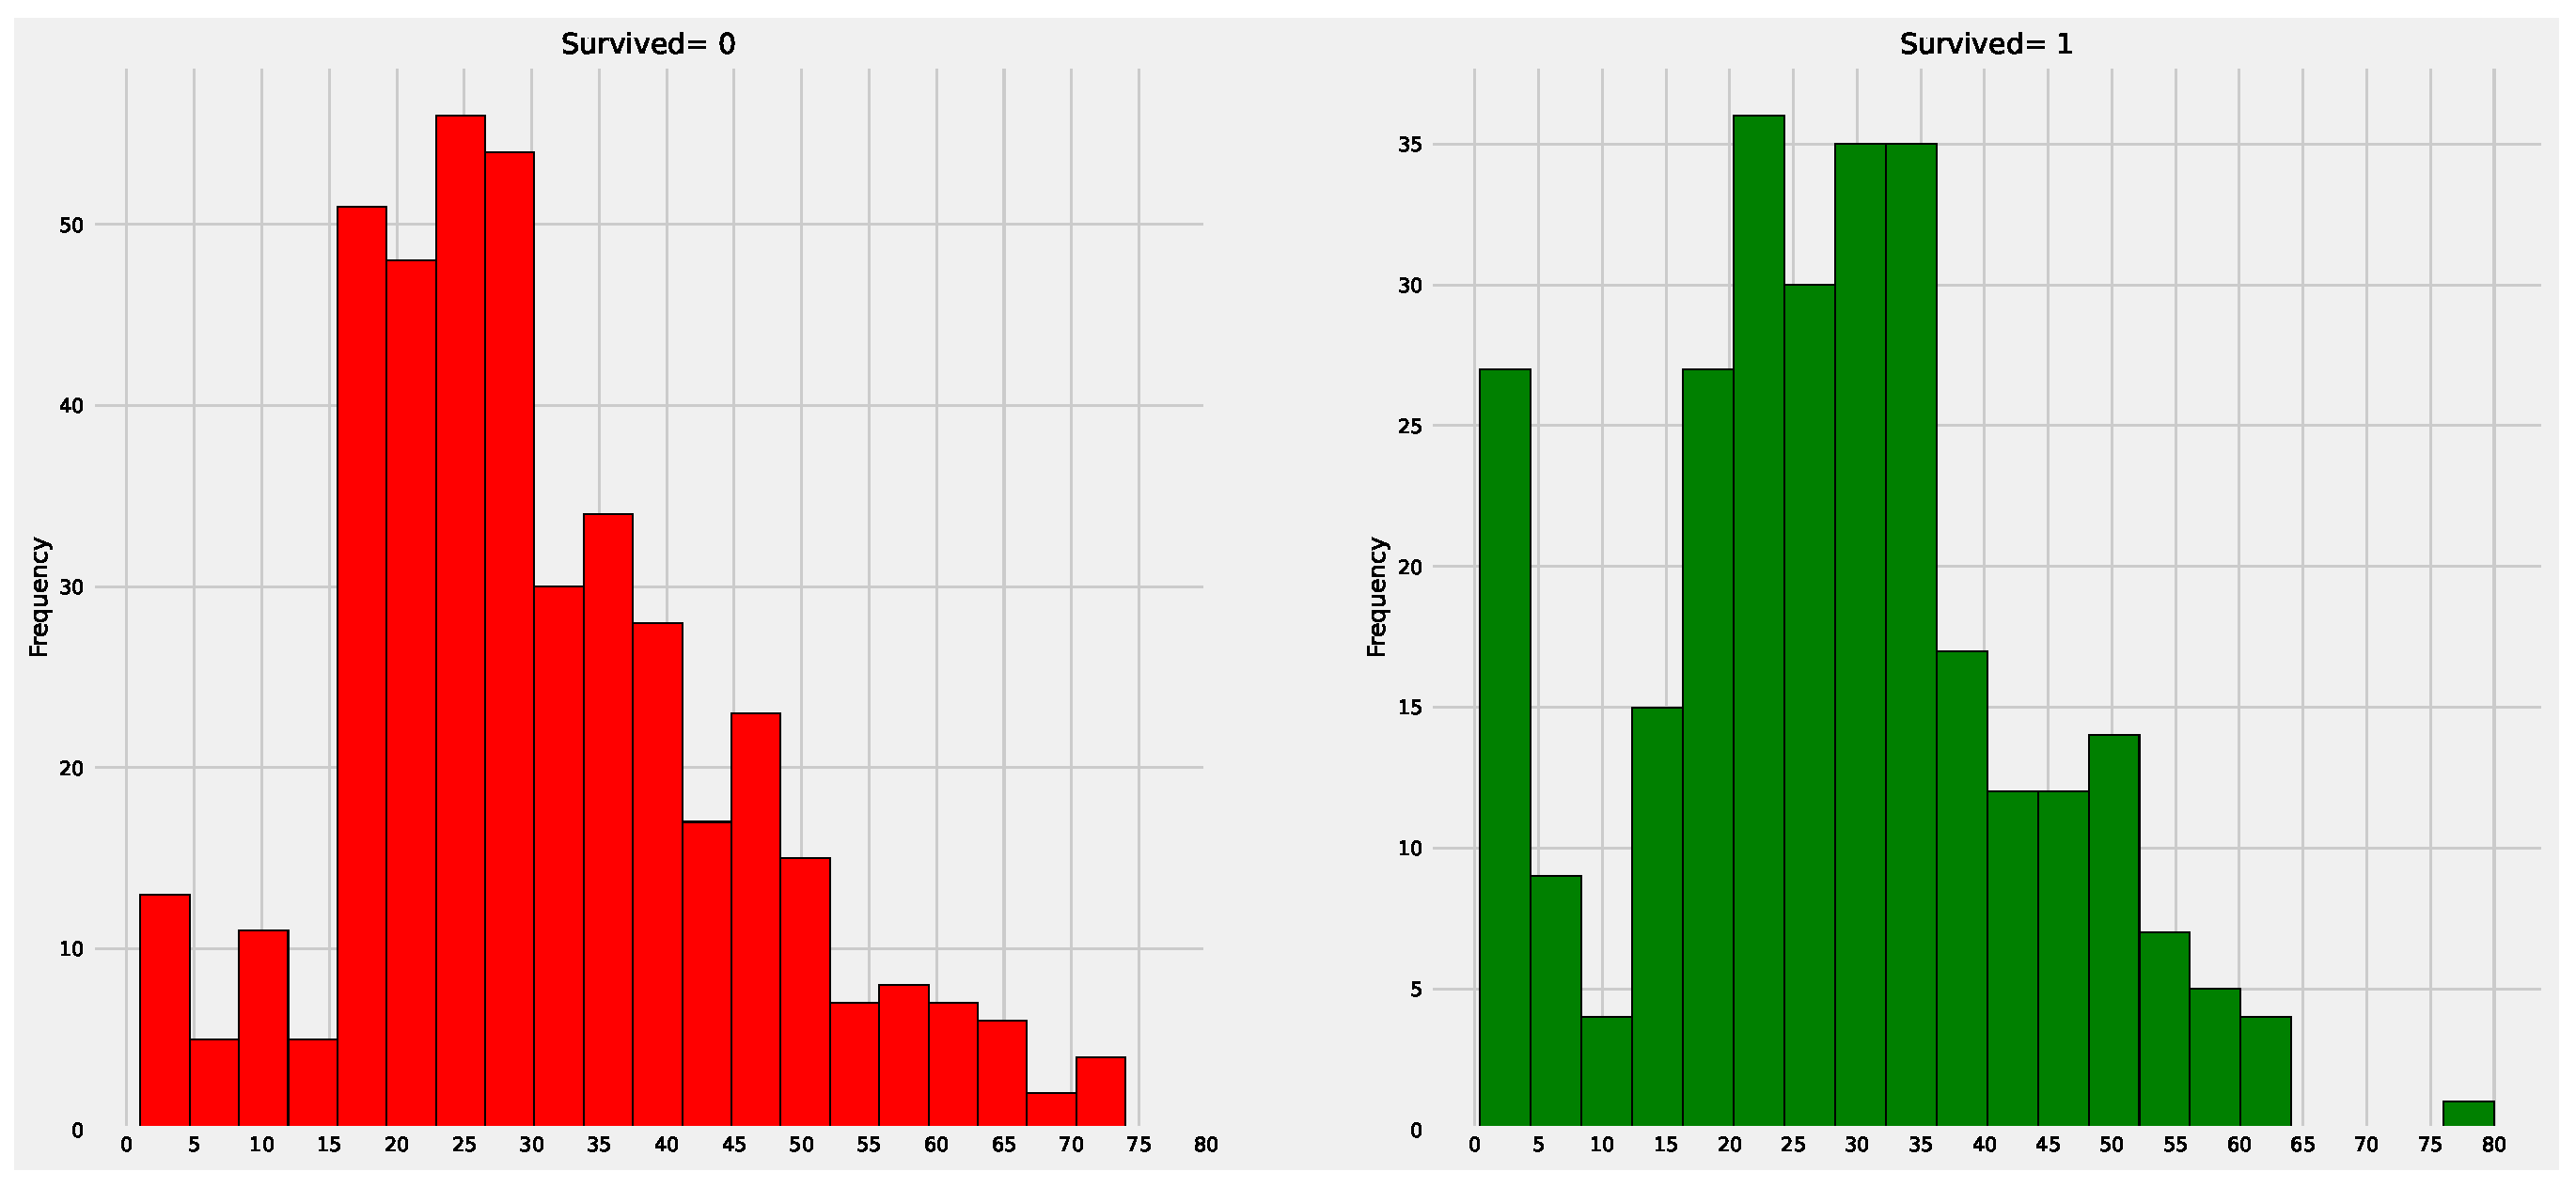
\includegraphics[width=0.6\textwidth,height=.2\textwidth]{/Users/pratikshyaparajuli/Desktop/kaggle/KaggleProject/Code/templatex/graphics/titanicimg/age.eps}
    }
  \caption{Survival rate with Age }\label{fig:age}
\end{figure}
\textcolor{orange}{Observations:}\\
1)The Toddlers(age<5) were saved in large numbers.\\
2)The oldest Passenger was saved(80 years).\\
3)Maximum number of deaths were in the age group of 30-40.
\end{slide}
%%
%%
\begin{slide}[toc=,bm=]{Embarked - Categorical Value}
  1)Maximum passenegers boarded from S. Majority of them being from Pclass3.\\
2)The Passengers from C survived. \\
3)The Embark S looks to the port from where majority of the rich people boarded. Still the chances for survival is low here.\\
4)Port Q had almost 95 percent of the passengers were from Pclass3.
\vspace{0.1cm}
\begin{figure}
  \centering
  \centerline{
    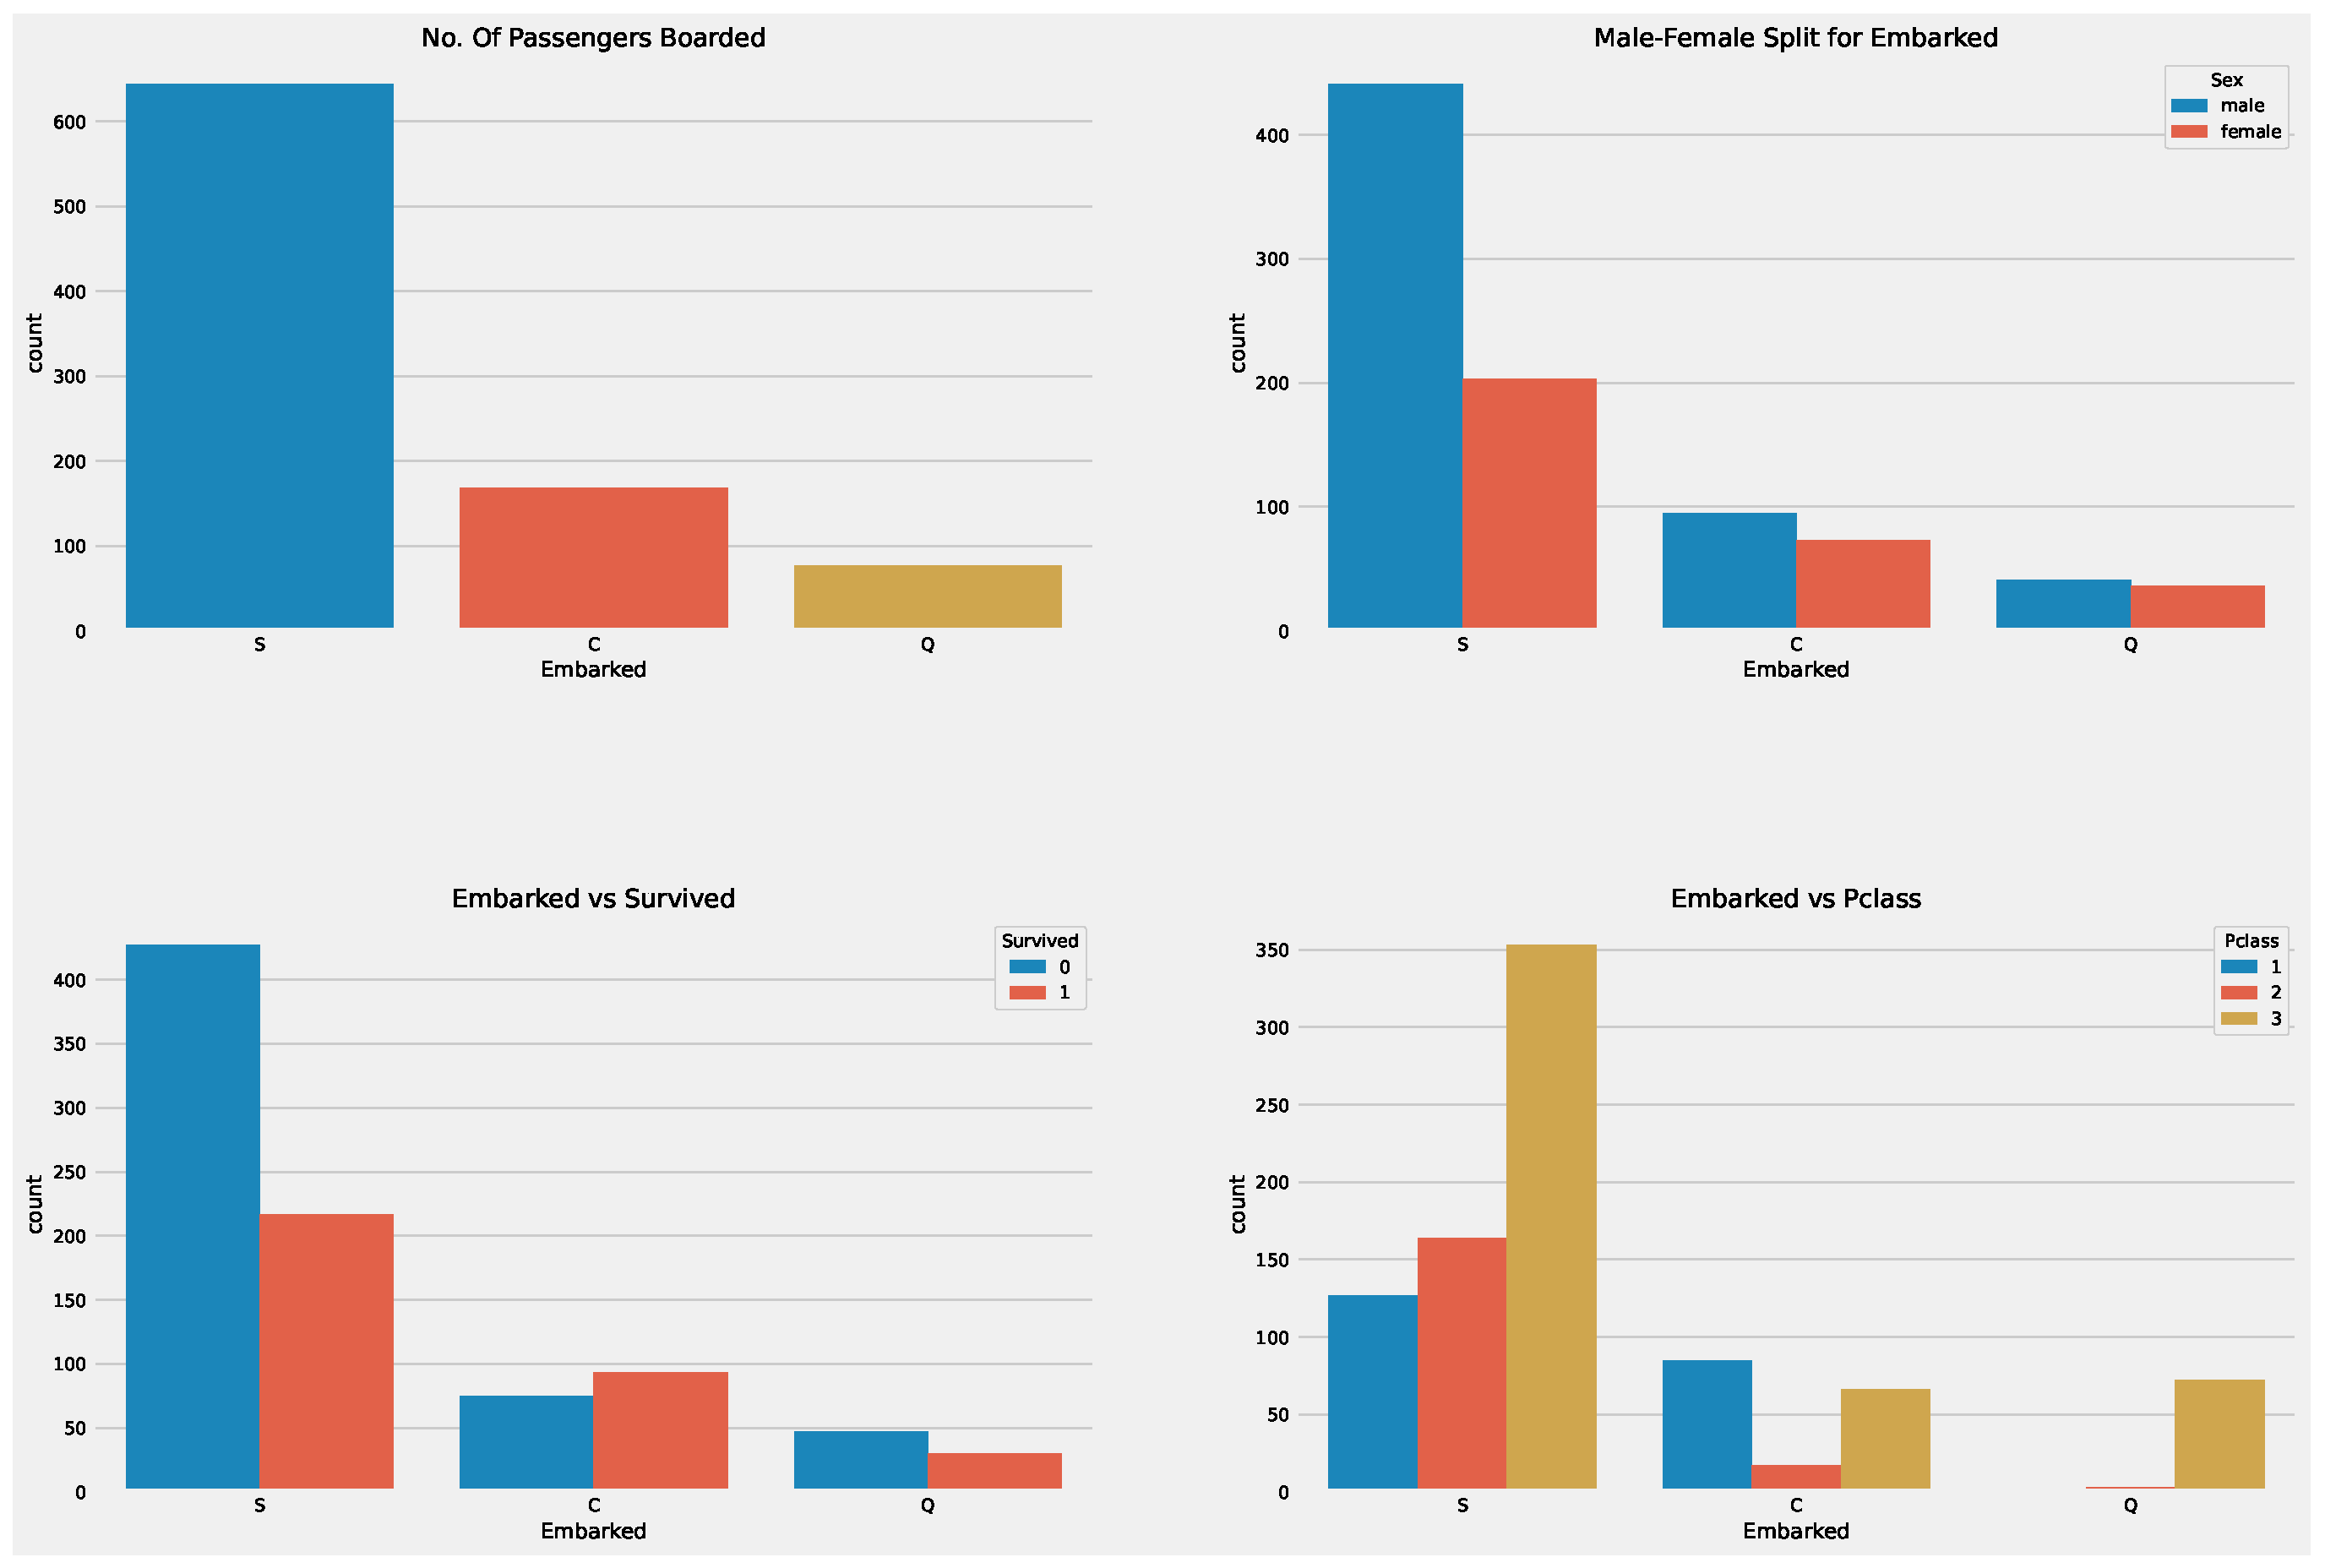
\includegraphics[width=0.6\textwidth,height=.3\textwidth]{/Users/pratikshyaparajuli/Desktop/kaggle/KaggleProject/Code/templatex/graphics/titanicimg/embark.eps}
    }
  \caption{Survival rate with Port of Embarkation}\label{fig:embark}
\end{figure}

\end{slide}
%%
%%
% \begin{slide}[toc=,bm=]{SibSip - Discrete Feature}
%   This feature represents whether a person is alone or with his family members.\\
%   Sibling = brother, sister, stepbrother, stepsister\\
%   Spouse = husband, wife\\
%   insert figure 4 bar graphs
% %\vspace{0.1cm}
% \begin{figure}
%   \centering
%   \selectcolormodel{rgb}
%   \missingfigure{Testing a long text string.}
%   %\includegraphics[width=0.6\textwidth]{figures//example-basketball-projection.eps}\\
%   \caption{Group Outlying Aspects Target}\label{fig:GroupOutAspect-target}
% \end{figure}
% \end{slide}
%%
%%
% \begin{slide}[toc=,bm=]{Parch - Discrete Feature}
%   Here too the results are quite similar. Passengers with their parents onboard have greater chance of survival. It however reduces as the number goes up.\\
% The chances of survival is good for somebody who has 1-3 parents on the ship. Being alone also proves to be fatal and the chances for survival decreases when somebody has >4 parents on the ship.
%   insert figure 4 bar graphs
% %\vspace{0.1cm}
% \begin{figure}
%   \centering
%   \selectcolormodel{rgb}
%   \missingfigure{Testing a long text string.}
%   %\includegraphics[width=0.6\textwidth]{figures//example-basketball-projection.eps}\\
%   \caption{Group Outlying Aspects Target}\label{fig:GroupOutAspect-target}
% \end{figure}
% \end{slide}
%%
%%
% \begin{slide}[toc=,bm=]{Fare - Continuous Feature}
%   Highest Fare was: 512.3292\\
%   Lowest Fare was: 0.0\\
%   Average Fare was: 32.2042079685746\\
%   insert figure graphs
% %\vspace{0.1cm}
% \begin{figure}
%   \centering
%   \selectcolormodel{rgb}
%   \missingfigure{Testing a long text string.}
%   %\includegraphics[width=0.6\textwidth]{figures//example-basketball-projection.eps}\\
%   \caption{Group Outlying Aspects Target}\label{fig:GroupOutAspect-target}
% \end{figure}
% \end{slide}
%%
%%
% \begin{slide}[toc=,bm=]{Observations in a Nutshell for all features}
%   Sex: The chance of survival for women is high as compared to men.\\
%   Pclass:There is a visible trend that being a 1st class passenger gives you better chances of survival. The survival rate for Pclass3 is very low. For women, the chance of survival from Pclass1 is almost 1 and is high too for those from Pclass2. Money Wins!!!.\\
%   Age: Children less than 5-10 years do have a high chance of survival. Passengers between age group 15 to 35 died a lot.\\
%   Embarked: This is a very interesting feature. The chances of survival at C looks to be better than even though the majority of Pclass1 passengers got up at S. Passengers at Q were all from Pclass3.\\
%   Parch+SibSp: Having 1-2 siblings,spouse on board or 1-3 Parents shows a greater chance of probablity rather than being alone or having a large family travelling with you.

% \end{slide}
%%
%%==========================================================================================


%%==========================================================================================
%%
%\begin{slide}[toc=,bm=]{Relation Between The Features}
%\vspace{0.1cm}
%\begin{figure}
  %\centering
  %\selectcolormodel{rgb}
  %\centerline{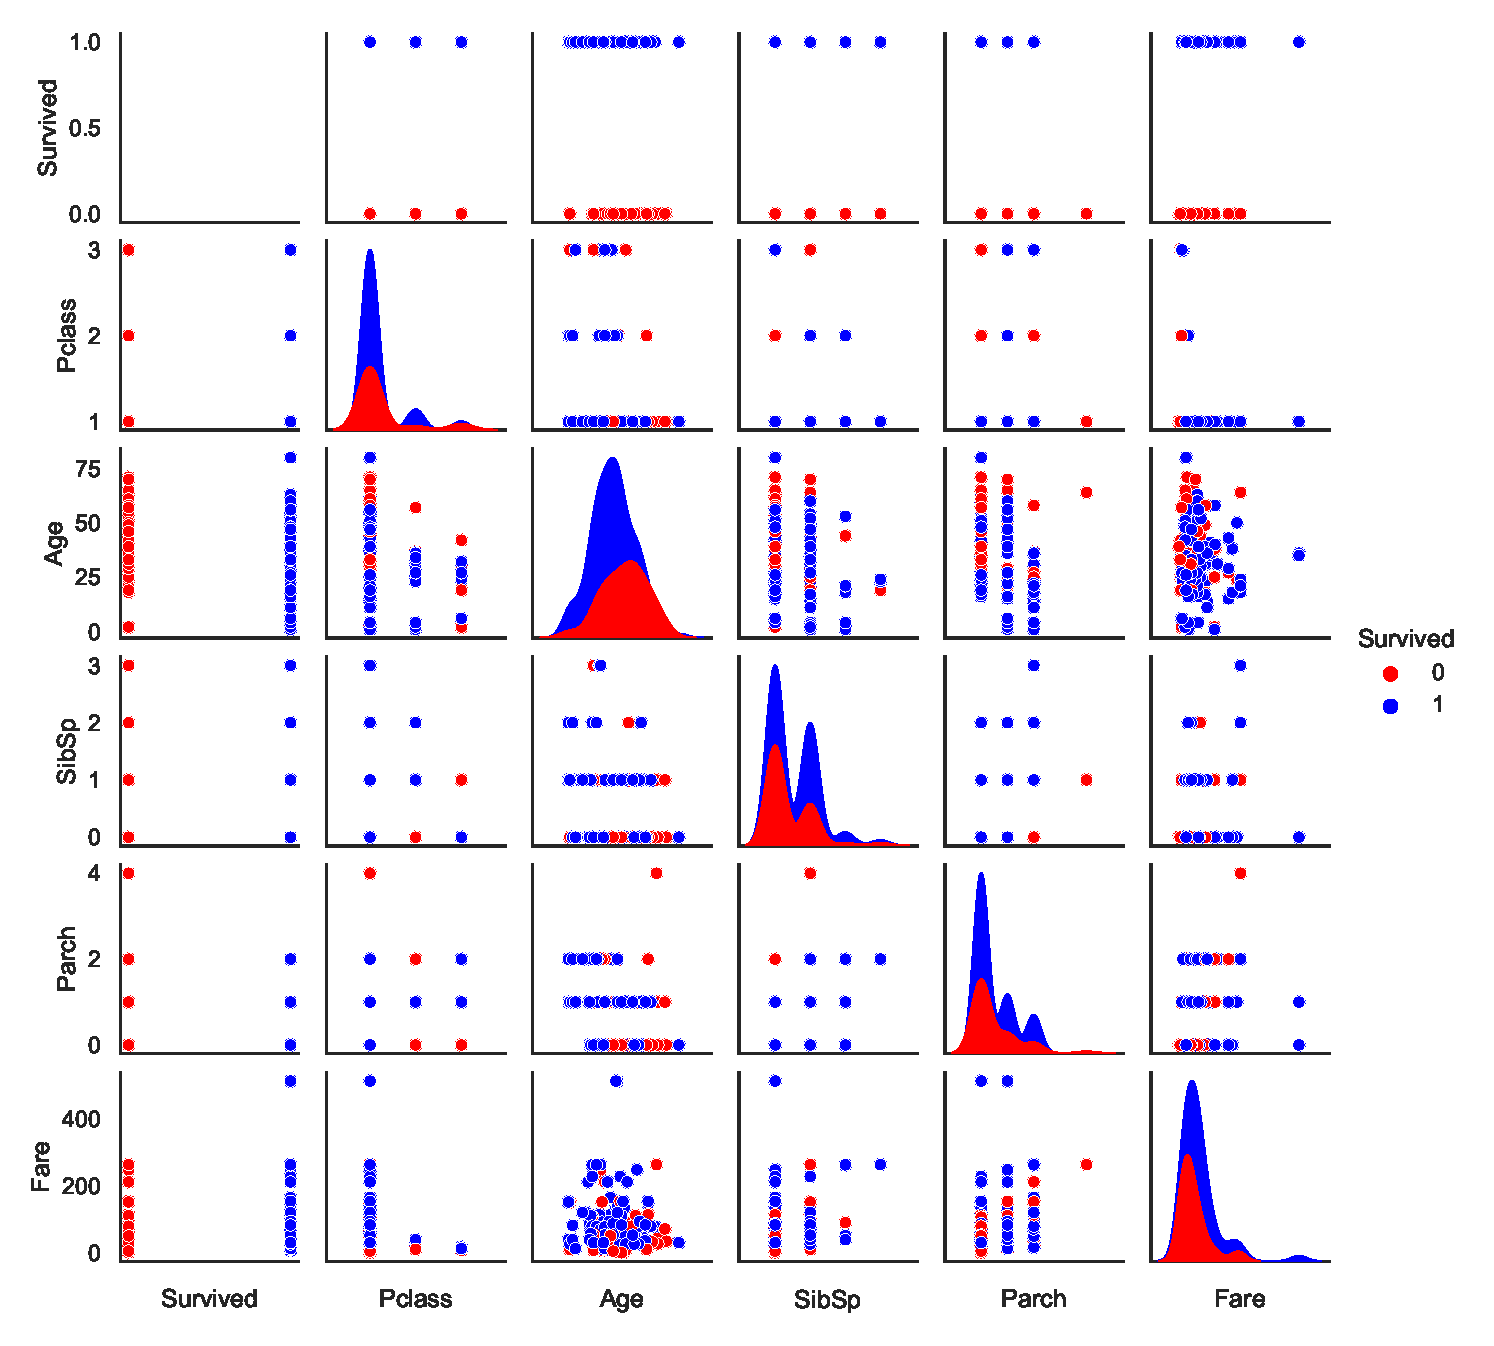
\includegraphics[scale=0.5,width=1.1\textwidth,height=0.4\textwidth]{/Users/pratikshyaparajuli/Desktop/kaggle/KaggleProject/Code/templatex/graphics/titanicimg/relation-between-features.eps}}
  %\caption{Relation Between The Features}\label{fig:Relation Between Features}
%\end{figure}
%\end{slide}
%%
%%==========================================================================================


%%==========================================================================================
%%
\begin{slide}[toc=,bm=]{Correlatoin Matrix}
 The highest correlation is between \textcolor{orange}{SibSp and Parch i.e 0.41.}
  %\vspace{0.1cm}
  \begin{figure}
    \centering
    %\selectcolormodel{rgb}
    \centerline{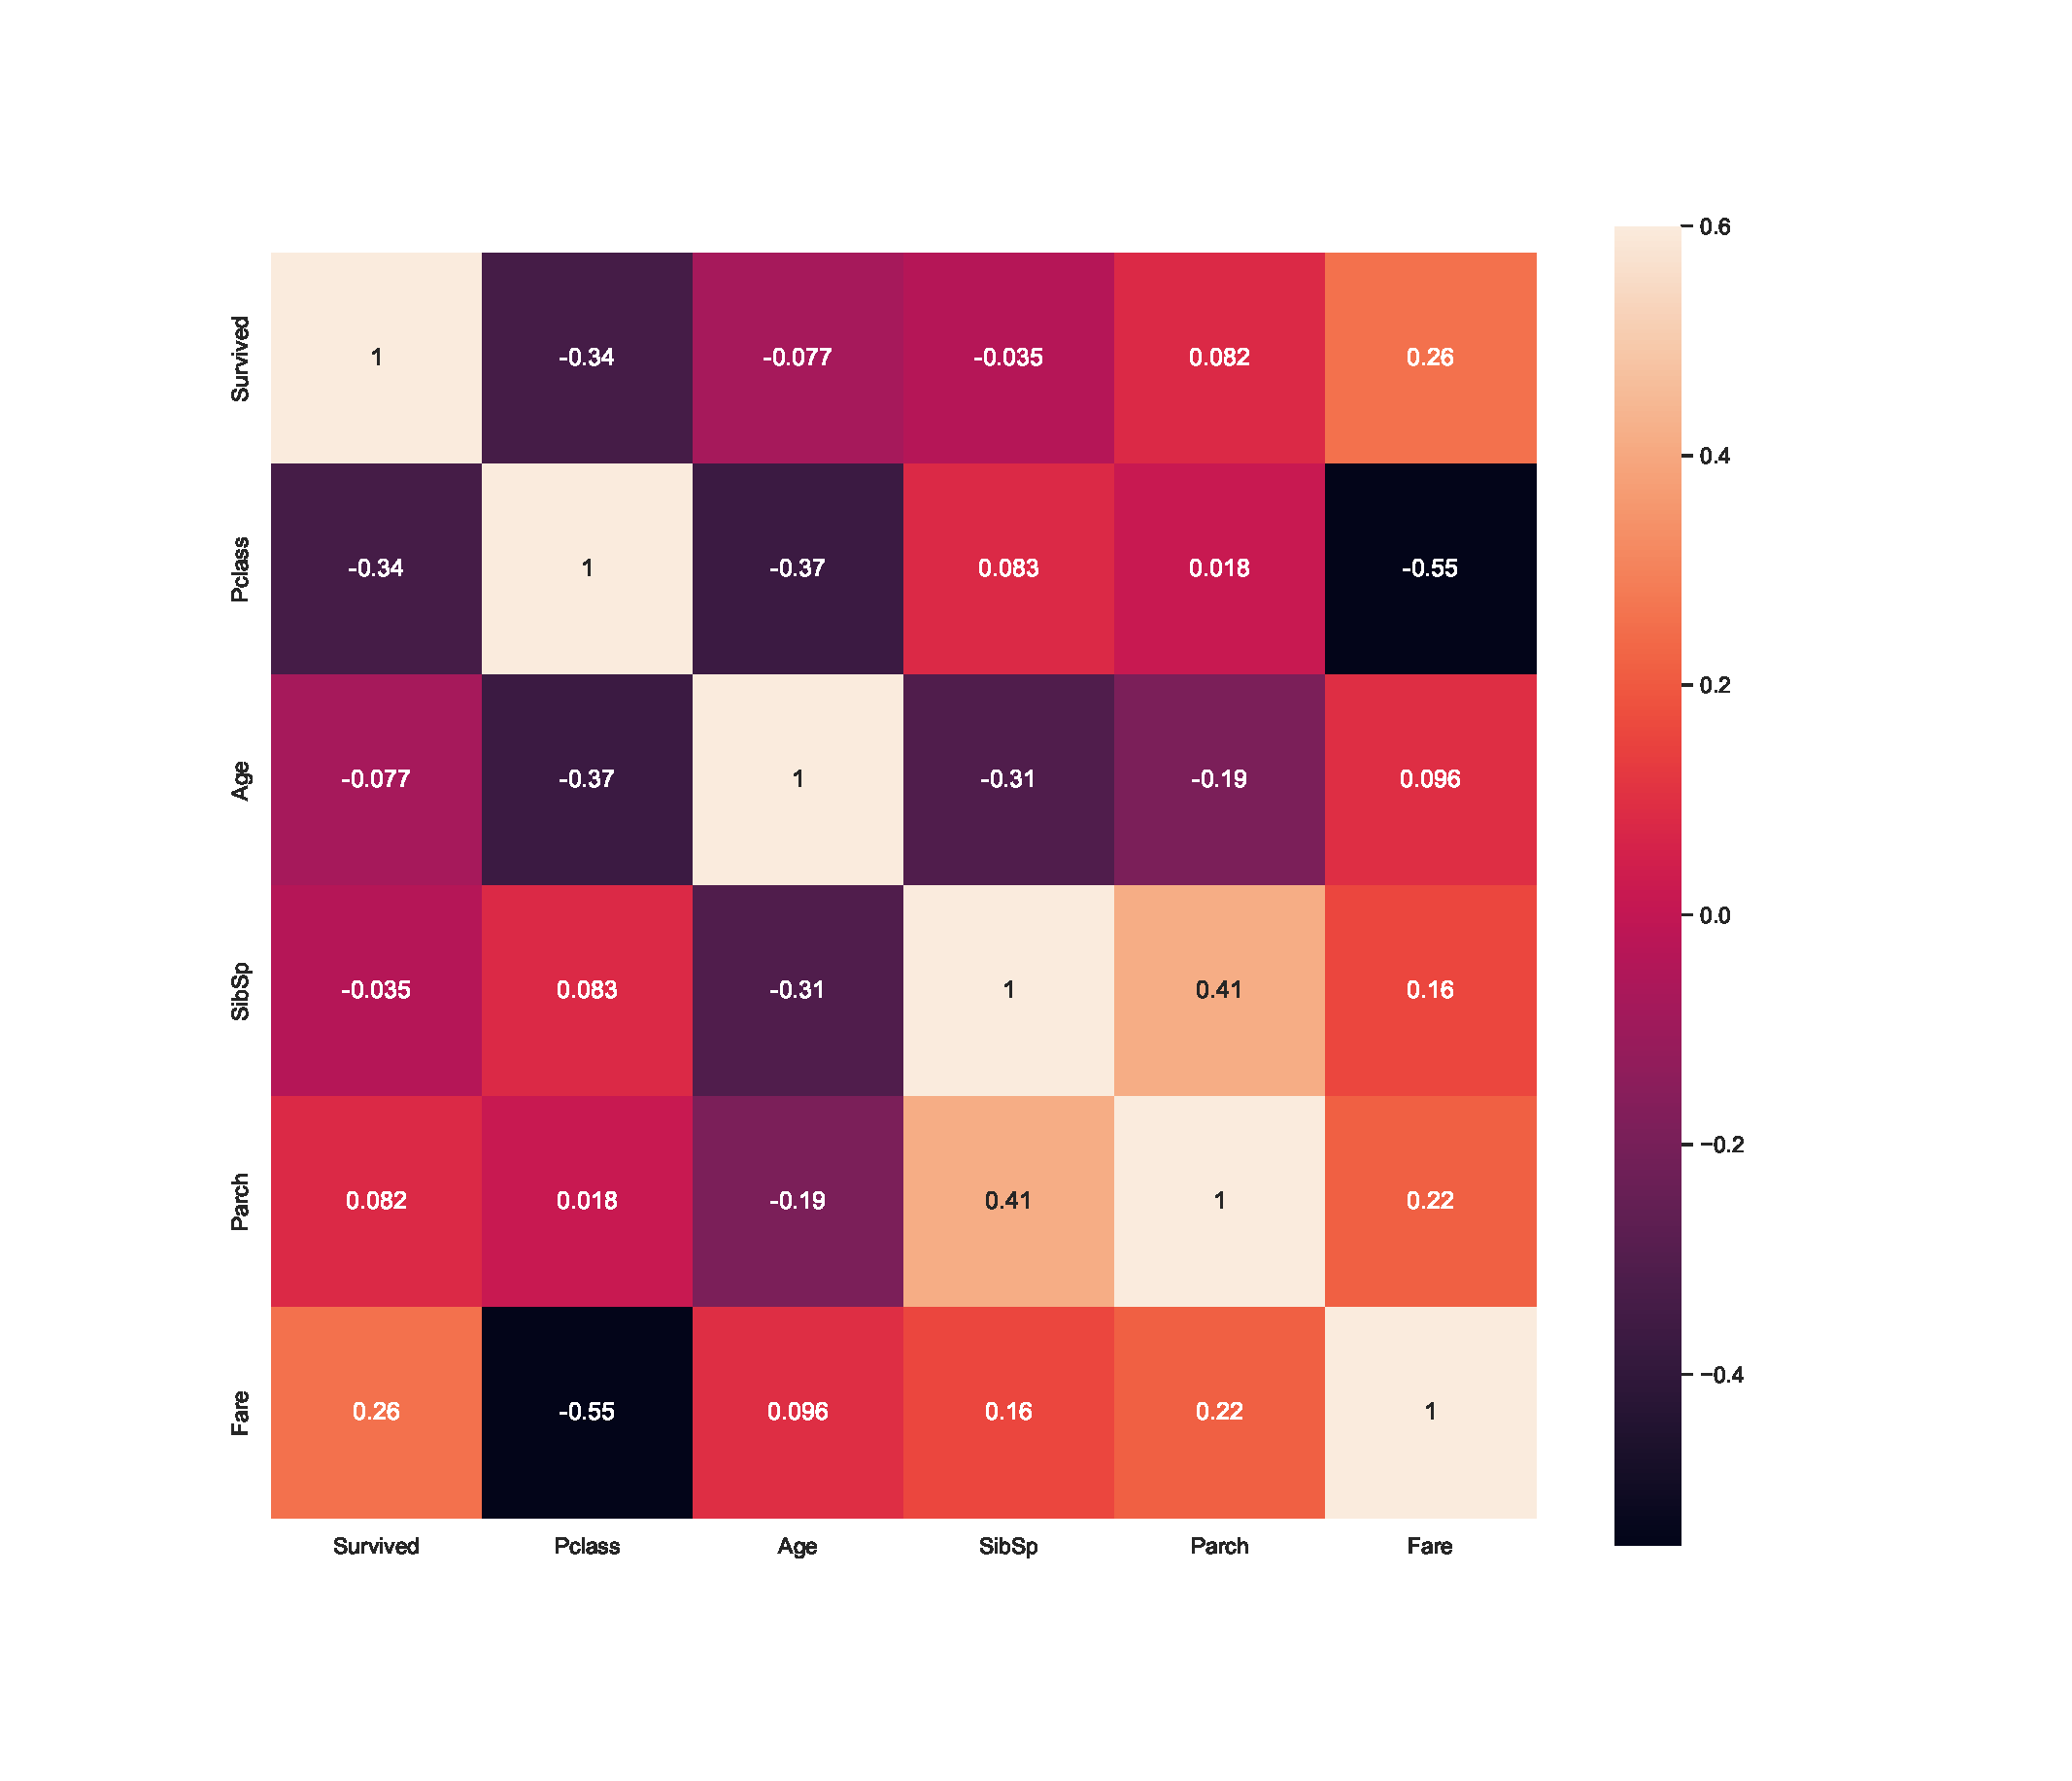
\includegraphics[scale=0.4,width=1.1\textwidth,height=0.5\textwidth]{/Users/pratikshyaparajuli/Desktop/kaggle/KaggleProject/Code/templatex/graphics/titanicimg/heatmap.eps}}
    \caption{Interpreting the heatmap}\label{fig:Heat map}
  \end{figure}
  \end{slide}
  %%
  %%==========================================================================================
  
  
  %%==========================================================================================
  %%
% \begin{slide}{Finding any relations or trends considering multiple features}
% %Challenges (1)
% \begin{itemize}
% \item
% How to \textcolor{orange}{represent} the group features.

% \begin{itemize}
% \item
% Can be affected by outlier values.

% \item
% Can \textcolor{orange}{Not} reflect the overall distribution of group features.
% \end{itemize}
% \end{itemize}

% %%==========================================================================================
% % \begin{note}
% % Based on current existing methods,
% % there still remains some research challenges.

% % The first one is how to represent the group features
% % based on the features of the individuals in the group.

% % Although the arithmetic mean of all elements
% % in each feature can describe the features of one group.
% % It can be affected by outlier values,
% % and can't reflect the entire distribution of group features.L
% % \end{note}
% %%==========================================================================================

% \end{slide}
%%
%%==========================================================================================


%%==========================================================================================
%%
% \begin{slide}[toc=,bm=]{Challenges (2)}

% \begin{itemize}
% \item
% How to \textcolor{orange}{evaluate} the outlying degree in different aspects.

% \begin{itemize}
% \item
% Need design a scoring function when necessary.

% \item
% Adopting an appropriate scoring function (without dimension bias) remains a problem.

% \end{itemize}
% \end{itemize}

% %%==========================================================================================
% \begin{note}
% The second challenge is how to evaluate the outlying degree of
% the query group between different aspects.

% In that case,
% we need to design a scoring function to measure the outlying degree.
% But adopting an appropriate scoring function without dimension bias still remains a problem.
% \end{note}
% %%==========================================================================================

% \end{slide}
%%
%%==========================================================================================
%%==========================================================================================
%%
% \begin{slide}[toc=,bm=]{Challenges (3)}

% \begin{itemize}
% \item
% How to \textcolor{orange}{improve} the efficiency.

% \begin{itemize}

% \item
% When the dimension of the \textcolor{orange}{data is high},
% the candidate subspace grows exponentially.

% \item
% It will easily go beyond the limits of the computation resources.

% \end{itemize}
% \end{itemize}

% %%==========================================================================================
% \begin{note}
% The third challenge is how to improve efficiency.

% To be specific,
% when the dimension of data is high,
% the candidate subspace increase dramatically,
% so that it is very easy to exceed the limit of computer resources.
% \end{note}
% %%==========================================================================================

% \end{slide}
%%
%%==========================================================================================


 \section{Feature Engineering and Data Cleaning}


%%==========================================================================================
%%
\begin{slide}[toc=,bm=]{Converting features into suitable form for modeling}
\begin{itemize}
  \item
   Age: Age_band
  \item 
  Family_size and Alone: Summation of Parch and SibSp
  \item  
  Fare: Fare_cat
\end{itemize}
\smallskip
  \twocolumn[
\savevalue{lfrheight}=7.6cm,
\savevalue{lfrprop}={
linestyle=solid,framearc=.2,linewidth=1pt},
rfrheight=\usevalue{lfrheight},
rfrprop=\usevalue{lfrprop}
]{
  \begin{table}[tb]
    \setlength{\abovecaptionskip}{0pt}
    \setlength{\belowcaptionskip}{10pt}
    %\centering
    \caption{Age_Band}
    
    \begin{tabular}{p{2.5cm}p{2.9cm}}
    \hline
      Age_band  & Numbers \\
    \hline
       1    & 382 \\
       2    & 325 \\
       0    & 104 \\
       3    & 69  \\
       4    & 11  \\
    \hline
    \end{tabular}
    \end{table}
}{
  \begin{figure}
    \centering
    %\selectcolormodel{rgb}
    \centerline{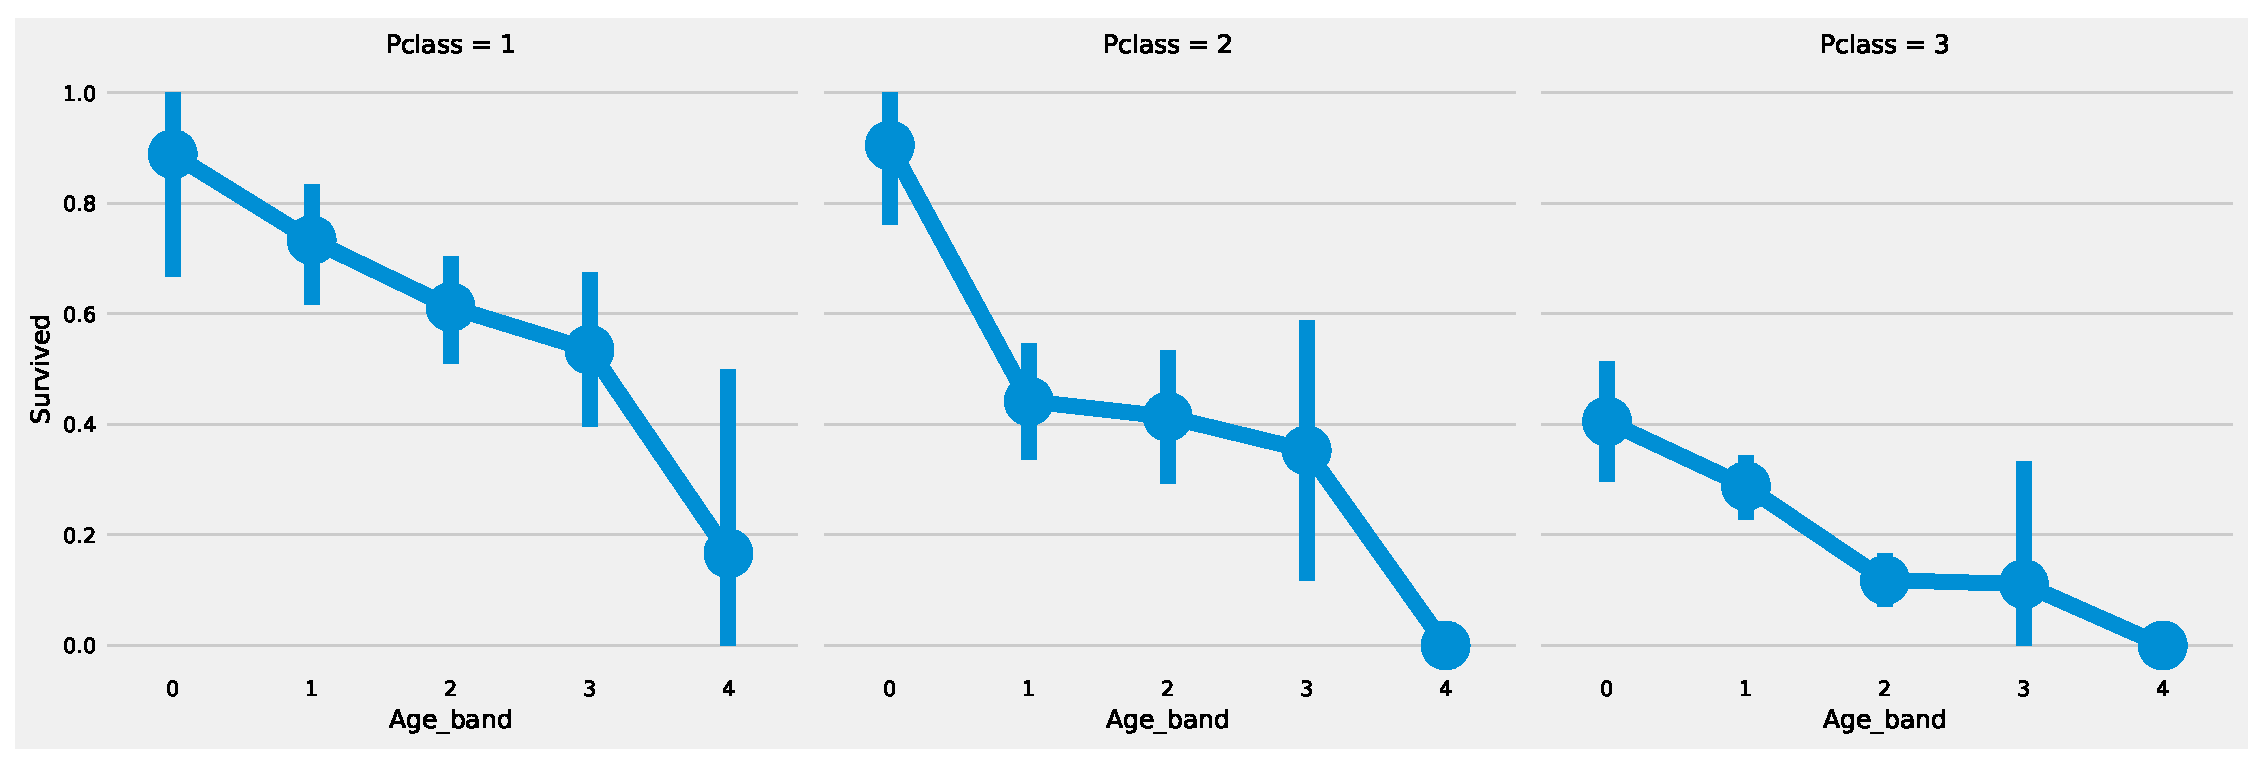
\includegraphics[scale=0.2,width=0.8\textwidth,height=0.5\textwidth]{/Users/pratikshyaparajuli/Desktop/kaggle/KaggleProject/Code/templatex/graphics/titanicimg/age-band.eps}}
    \caption{Age_Band}\label{fig:Age_Band}
  \end{figure}
}
%%==========================================================================================
% \begin{note}
% In order to tackle the above issues,
% GOAM algorithm is involved.

% Let's have a look at the framework of this algorithm.
% The first step is to use the histogram to represent the group features
% based on all individuals in the group.

% Following that,
% we utilize the earth mover distances to measure the
% outlying degree between groups.
% This is the second step:
% outlying degree scoring.

% The last step is to identify the outlying aspects.

% \end{note}
%%==========================================================================================

\end{slide}
%%
%%==========================================================================================


%%==========================================================================================
%%
\begin{slide}{Removing Redundant features}
%Step One - Group Feature Extraction}
\begin{itemize}
\item
  Name--> We don't need name feature as it cannot be converted into any categorical value.
  \item
  Ticket--> It is any random string that cannot be categorised.
  \item
  Fare--> We have the Fare_cat feature, so unneeded
  \item
   Cabin--> A lot of NaN values and also many passengers have multiple cabins. So this is a useless feature.
  \item
   Fare_Range--> We have the fare_cat feature.
  \item
  PassengerId--> Cannot be categorised.
\end{itemize}
\end{slide}
%%
%%==========================================================================================
\begin{slide}{Correlation Matrix after Data Cleaning}
  Positive correlation: \textcolor{orange}{SibSp andd Family_Size and Parch and Family_Size} and Negative correlation: \textcolor{orange}{Alone and Family_Size}
   %\vspace{0.1cm}
   \begin{figure}
     \centering
     %\selectcolormodel{rgb}
     \centerline{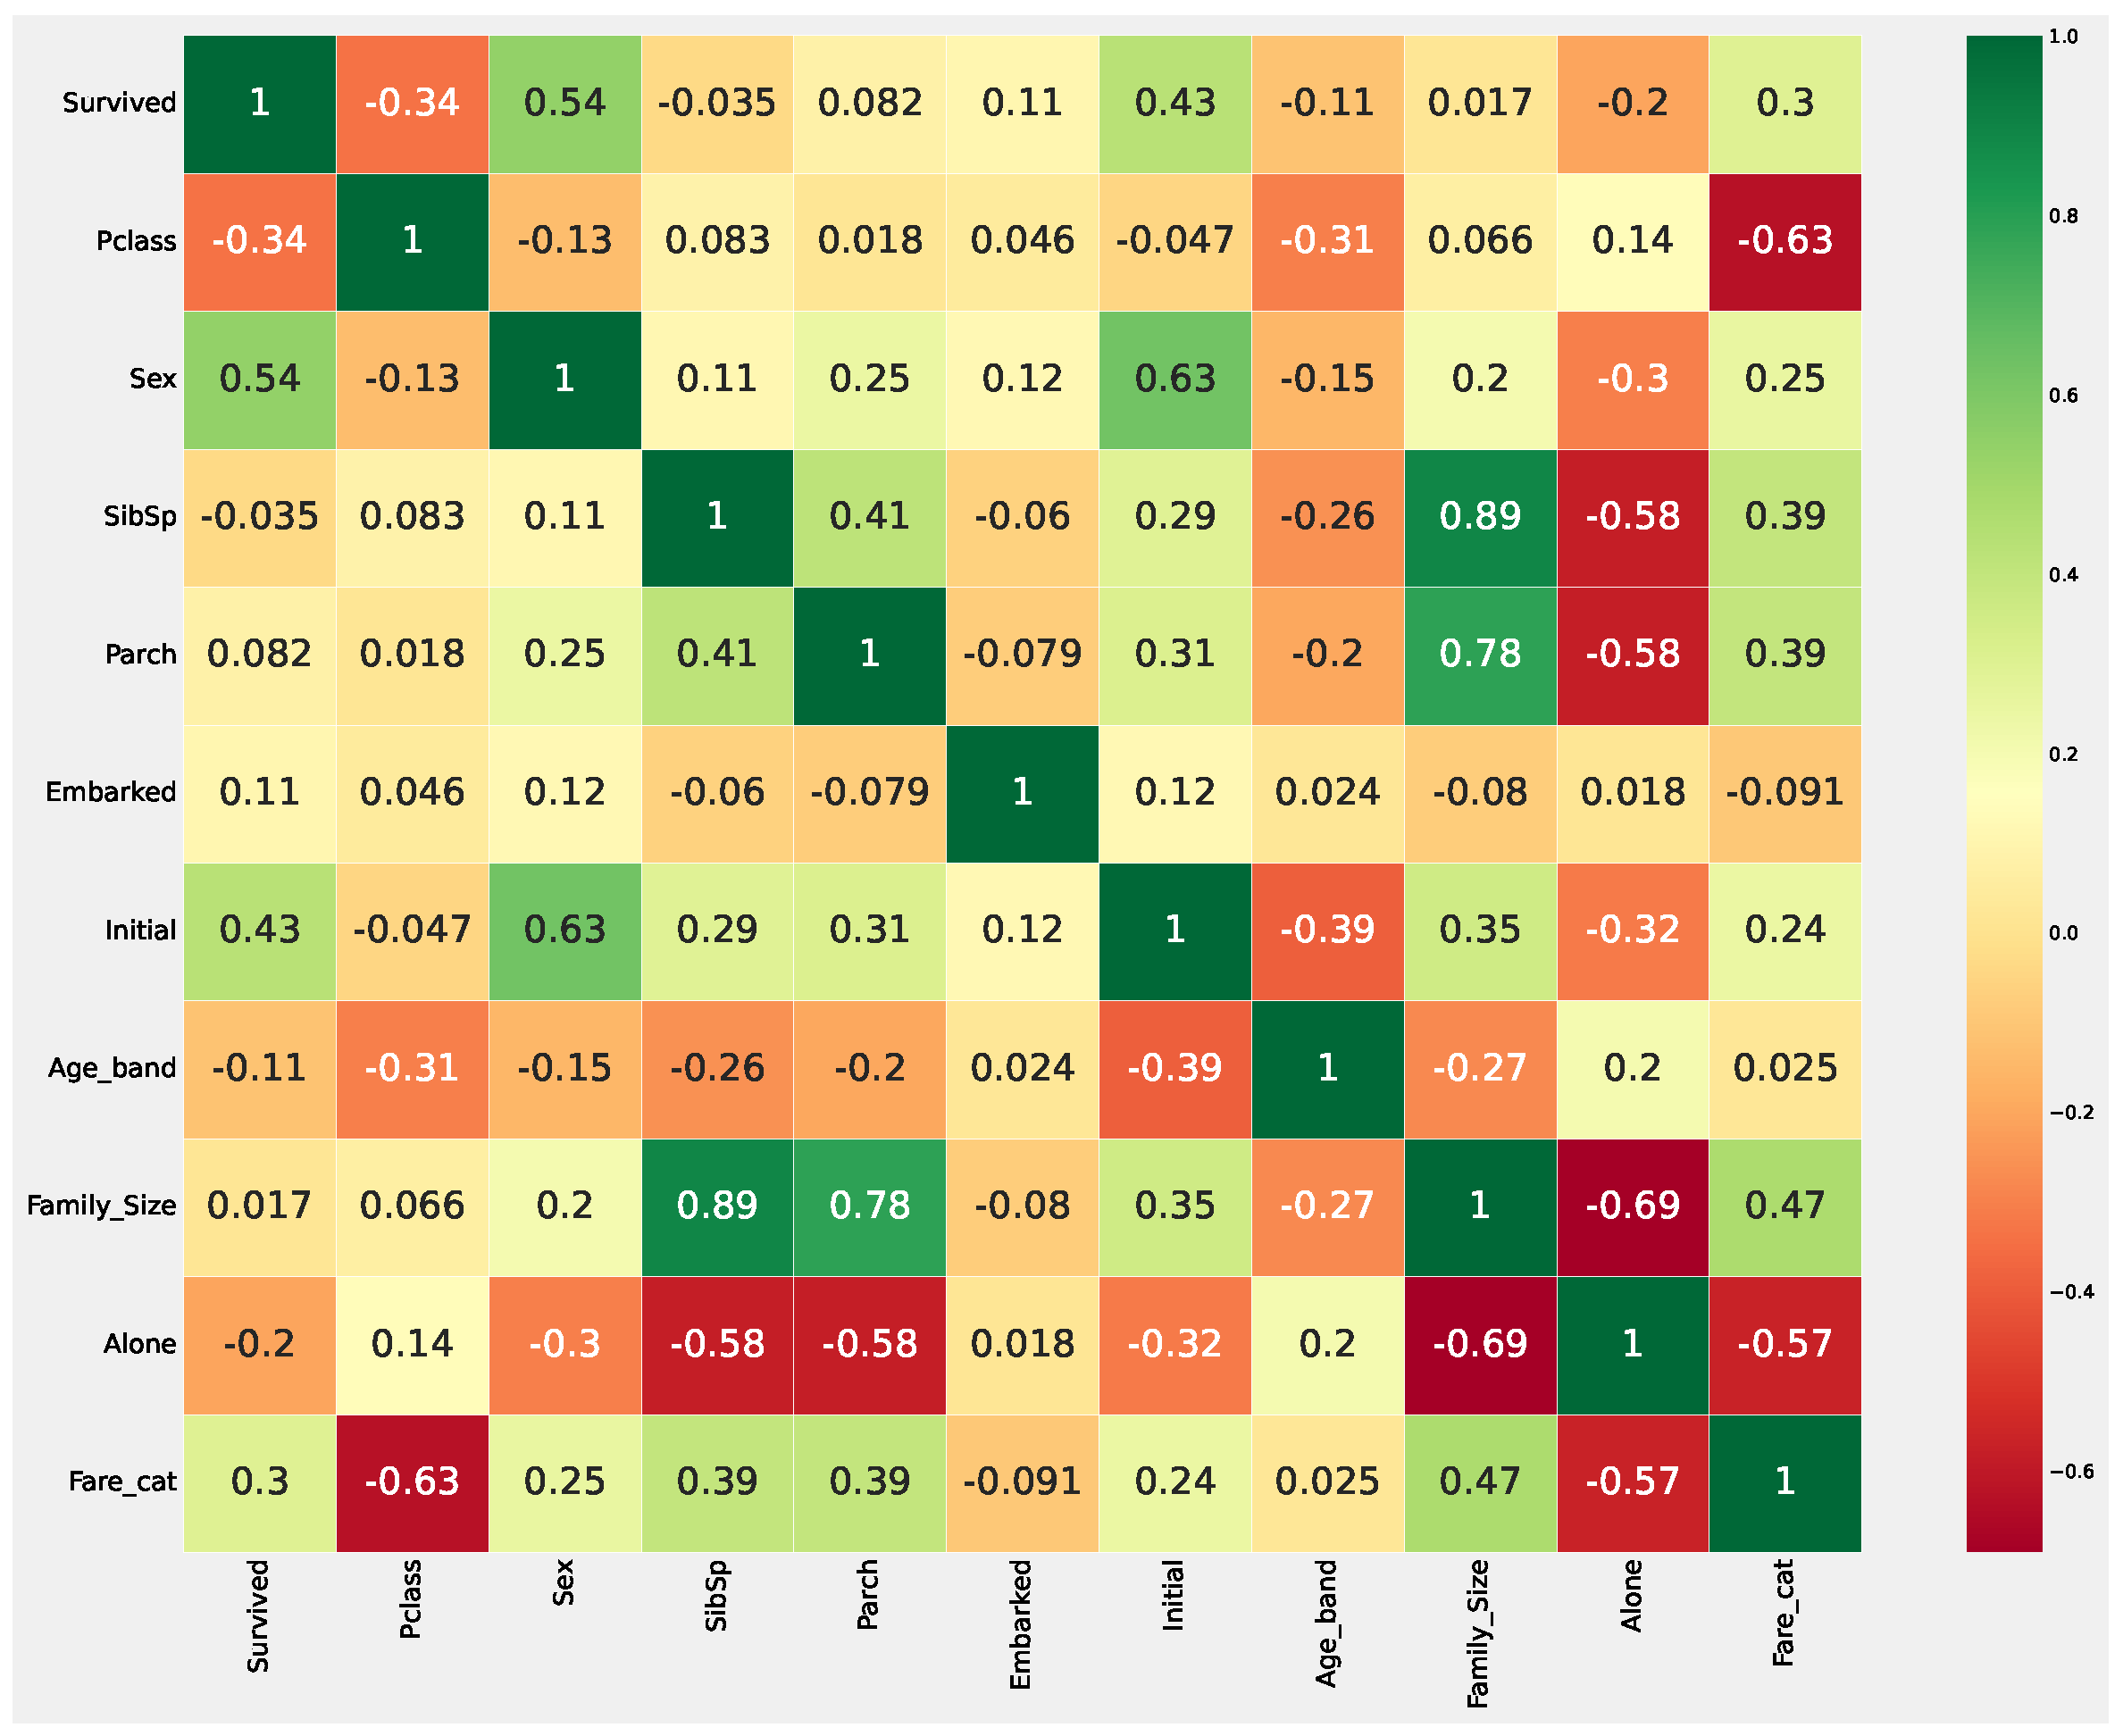
\includegraphics[scale=0.4,width=1.1\textwidth,height=0.45\textwidth]{/Users/pratikshyaparajuli/Desktop/kaggle/KaggleProject/Code/templatex/graphics/titanicimg/clean-heatmap.eps}}
     \caption{Correlation Matrix after Data Cleaning}\label{fig:clean-Heat map}
   \end{figure}
   \end{slide}

\section{Predictive Modeling}


%%==========================================================================================
%%
\begin{slide}[toc=,bm=]{Evaluation Classification Algorithms}

\begin{center}
\begin{itemize}
\item
Logistic Regression
\item
Support Vector Machines (Linear and radial)
\item
Random Forest
\item
K-Nearest Neighbours
\item
Naive Bayes
\item
Decision Tree
\end{itemize}
\end{center}

%%==========================================================================================
% \begin{note}
% Before showing the experiment results,
% I will introduce the evaluation of the experiment.

% We use accuracy formula to make comparisons between GOAM algorithm
% and outlying aspect mining method.
% In the accuracy formula,
% P stands for identified outlying aspects;
% and T means the real outlying aspects.
% \end{note}
%%==========================================================================================

\end{slide}
%%
%%==========================================================================================


%%==========================================================================================
%%
\begin{slide}{Prediction Accuracy}

\begin{itemize}
\item 
   Split the train sample into train and test dataset
   \item 
   Train Data_size : 0.7 and Test Data_size : 0.3
   \item 
   Total sample size = 891; training sample size = 623, testing sample size = 268
  \end{itemize}

\begin{table}
\setlength{\abovecaptionskip}{0pt}
\setlength{\belowcaptionskip}{10pt}
\centering
\caption{Accuracy Comparison of different Classifier Algorithms}

\begin{tabular}{cccc}
  \toprule
  % after \\: \hline or \cline{col1-col2} \cline{col3-col4} ...
   & Acuracy \\
\midrule
  Radial Support Vector Machines(rbf-SVM)   & 0.835820895522388 \\
  Linear Support Vector Machine(linear-SVM) & 0.8171641791044776 \\
  Logistic Regression & 0.8134328358208955 \\
  Decision Tree & 0.8059701492537313 \\
  K-Nearest Neighbours(KNN) & 0.832089552238806 \\
  Gaussian Naive Bayes & 0.8134328358208955 \\
  Random Forests & 0.8208955223880597\\
\bottomrule
\end{tabular}
\end{table}

\end{slide}

%%==========================================================================================
%%
% \section{Evaluation Results}



% \begin{slide}[toc=,bm=]{Evaluation}

% \begin{center}
% \begin{itemize}

% \item
% \smallskip
% \large
% {$Accuracy = \frac{P}{T}$ \\
% P: Identified outlying aspects \\

% T: Real outlying aspects}

% \end{itemize}
% \end{center}

% %%==========================================================================================
% \begin{note}
% Before showing the experiment results,
% I will introduce the evaluation of the experiment.

% We use accuracy formula to make comparisons between GOAM algorithm
% and outlying aspect mining method.
% In the accuracy formula,
% P stands for identified outlying aspects;
% and T means the real outlying aspects.
% \end{note}
% %%==========================================================================================

% \end{slide}
%%
%%==========================================================================================


%%==========================================================================================
%%
% \begin{slide}{Synthetic Dataset}

% \begin{itemize}
% \item Synthetic Dataset and Ground Truth
% \end{itemize}

% \begin{table}
% \setlength{\abovecaptionskip}{0pt}
% \setlength{\belowcaptionskip}{10pt}
% \centering
% \caption{Synthetic Dataset and Ground Truth}

% \begin{tabular}{p{2.8cm}p{0.9cm}p{0.9cm}p{0.9cm}p{0.9cm}p{0.9cm}p{0.9cm}p{0.9cm}p{0.9cm}}
% \hline
%   % after \\: \hline or \cline{col1-col2} \cline{col3-col4} ...
%   Query group  & $\mathbf{F_1}$ & $\mathbf{F_2}$ & $F_3$ & $\mathbf{F_4}$ & $F_5$ & $F_6$ & $F_7$ & $F_8$\\
% \hline
%   $i_1$   & \bf{10} & \bf{8}  & 9  & \bf{7}  & 7 & 6 & 6  & 8\\
%   $i_2$   & \bf{9}  & \bf{9}  & 7  & \bf{8}  & 9 & 9 & 8  & 9\\
%   $i_3$   & \bf{8}  & \bf{10} & 8  & \bf{9}  & 6 & 8 & 7  & 8\\
%   $i_4$   & \bf{8}  & \bf{8}  & 6  & \bf{7}  & 8 & 8 & 6  & 7\\
%   $i_5$   & \bf{9}  & \bf{9}  & 9  & \bf{7}  & 7 & 7 & 8  & 8\\
%   $i_6$   & \bf{8}  & \bf{10} & 8  & \bf{8}  & 6 & 6 & 8  & 7\\
%   $i_7$   & \bf{9}  & \bf{9}  & 7  & \bf{9}  & 8 & 8 & 8  & 7\\
%   $i_8$   & \bf{10} & \bf{9}  & 10 & \bf{7}  & 7 & 7 & 7  & 7\\
%   $i_9$   & \bf{9}  & \bf{10} & 8  & \bf{8}  & 7 & 6 & 7  & 7\\
%   $i_{10}$& \bf{9}  & \bf{9}  & 7  & \bf{7}  & 7 & 8 & 8  & 8\\
% \hline
% \end{tabular}
% \end{table}

% %%==========================================================================================
% \begin{note}
% Now,
% I am gonna use a synthetic dataset to verify our method.

% The dataset we used in our experiment contains $10$ groups,
% each group consists of $10$ members,
% and each member has $8$ features: $F_1$ to $F_8$.

% Table $5$ shows the original data of one group,
% and the bold features represent the ground truth,
% The ground truth include trivial outlying feature \{$F_1$\},
% and non-trivial outlying subspace \{$F_2$, $F_4$\}.
% \end{note}
% %%==========================================================================================

% \end{slide}
%%
%%==========================================================================================


%%==========================================================================================
%%
% \begin{slide}[toc=,bm=]{Synthetic Dataset Results}

% \begin{table}[tb]
% \setlength{\abovecaptionskip}{0pt}
% \setlength{\belowcaptionskip}{10pt}
% \centering
% \caption{The experiment result on synthetic dataset}

% \begin{tabular}{ c | c | c | c }
% \toprule
%   % after \\: \hline or \cline{col1-col2} \cline{col3-col4} ...
%   Method     &  Truth Outlying Aspects    & Identified Aspects & Accuracy      \\
% \midrule
%   GOAM       &  $\{F_1\}$, $\{F_2F_4\}$   &  $\{F_1\}$, $\{F_2F_4\}$    & 100\%    \\

% Arithmetic Mean based OAM &  $\{F_1\}$, $\{F_2F_4\}$   &  $\{F_4\}$, $\{F_2\}$    &  0\% \\

% Median based OAM &  $\{F_1\}$, $\{F_2F_4\}$   &  $\{F_2\}$, $\{F_4\}$    &           0\% \\
% \bottomrule
% \end{tabular}
% \end{table}

% %%==========================================================================================
% \begin{note}
% From table $6$,
% we can see that GOAM method can identify the trivial outlying features
% and non-trivial outlying subspaces accurately and
% it is obvious from the table that the accuracy of GOAM is the best,
% which is 100\%.

% This is because the outlying aspects mining method
% can't obtain the features of a group and the scoring function
% is based on point to point metric.
% Therefore,
% it is not suitable for group outlying aspects mining.
% \end{note}
% %%==========================================================================================

% \end{slide}
%%
%%==========================================================================================


%%==========================================================================================
%%
% \begin{slide}{NBA Dataset}
% Data Collection
% \begin{description}[type=1]
% \item
% Source\\
% \qquad
% \emph{Yahoo Sports} website (\url{http://sports.yahoo.com.cn/nba})

% \item
% Data

% \begin{itemize}
%  \item Extract NBA teams' data until March 30, 2018;
%  \item 6 divisions;
%  \item 12 features (eg: \emph{Point Scored}).
% \end{itemize}
% \end{description}

% %%==========================================================================================
% \begin{note}
% Next,
% I will illustrate it further by applying the GOAM algorithm to the NBA dataset.
% The data was collected from Yahoo Sports website.

% In our experiment,
% a web crawler was deployed to extract data
% for all NBA teams until March 30, 2018.
% The data includes all teams from the six divisions,
% and each player in the team has 12 features,
% such as point scored, field goal\dots
% \end{note}
% %%==========================================================================================

% \end{slide}
%%
%%==========================================================================================


%%==========================================================================================
%%
% \begin{slide}[toc=,bm=]{NBA Dataset}
% The detail features are as follows:

% \begin{table}[tb]
% \setlength{\abovecaptionskip}{0pt}
% \setlength{\belowcaptionskip}{10pt}
% \centering
% \caption{Collected data of Brooklyn Nets Team}

% \begin{tabular}{p{0.9cm}p{0.9cm}p{0.9cm}p{0.9cm}p{0.9cm}p{0.9cm}p{0.9cm}p{0.9cm}p{0.9cm}p{0.9cm}p{0.9cm}p{0.9cm}}
% \hline
%   Pts & FGA & FG\% & 3FA & 3PT\% & FTA & FT\% & Reb & Ass & To & Stl & Blk \\
% \hline
%   18   & 12    & 42 &2.00 & 50 & 7.00 & 100& 0& 4& 3& 0& 0 \\
%   15.7 & 14.07 & 41 &5.45 & 32 & 3.05 & 75 & 3.98& 5.1& 2.98& 0.69& 0.36\\
%   14.5 & 11.1  & 47 &0.82 & 26 & 4.87 & 78 & 6.82& 2.4& 1.74& 0.92& 0.66 \\
%   13.5 & 10.8  & 42 &5.37 & 37 & 3.38 & 77 & 6.66& 2& 1.38& 0.83& 0.42 \\
%   12.7 & 10.59 & 39 &5.36 & 33 & 3.37 & 82 & 3.24& 6.6& 1.56& 0.89& 0.31 \\
%   12.6 & 10.93 & 40 &6.94 & 37 & 1.70 & 84 & 4.27& 1.5& 1.06& 0.61& 0.44 \\
%   12.2 & 10.39 & 44 &3.42 & 35 & 2.70 & 72 & 3.79& 4.1& 2.15& 1.12& 0.32 \\
%   10.6 & 7.85  & 49 &4.51 & 41 & 1.35 & 83 & 3.34& 1.6& 1.15 & 0.45& 0.24 \\
% \hline
% \end{tabular}
% \end{table}

% %%==========================================================================================
% \begin{note}
% Table $7$ shows part of the collected data.
% From this table,
% we can see that the feature values are continuous.
% \end{note}
% %%==========================================================================================

% \end{slide}
%%
%%==========================================================================================


%%==========================================================================================
%%
% \begin{slide}[toc=,bm=]{NBA Dataset}
% \begin{itemize}
% \item Data Preprocess
% \end{itemize}

% \begin{table}
% \setlength{\abovecaptionskip}{0pt}
% \setlength{\belowcaptionskip}{10pt}
% \centering
% \caption{The bins that used to discrete data of each feature}

% \begin{tabular}{p{2.5cm}p{2cm}p{1.8cm}p{2cm}p{1.8cm}p{1.8cm}p{1.8cm}}
% \hline
%   Labels & Pts & FGA & FG\% & 3FA & 3PT\% & FTA  \\
% \hline
%   low &  [0,5]& [0,4] & [0,0.35] & [0,1.0] & [0,0.2] & [0,1.0] \\
%   medium& (5,10]& (4,7] & (0.35,0.45] & (1.0,2.5]& (0.2,0.3] & (1.0,1.5] \\
%   high &  (10,15] & (7,10] & (0.45,0.5] & (2.5,3.5]& (0.3,0.35]& (1.5,2.5] \\
%   very high&(15,$+\infty$]& (10,$+\infty$] & (0.5,1] & (3.5,$+\infty$] & (0.35,1] & (2.5,$+\infty$] \\
% \hline
%  Labels & FT\% & Reb & Ass & To & Stl & Blk \\
% \hline
%   low   & [0,0.6] & [0,2.0] & [0,1.0] & [0,0.6] & [0,0.2] & [0,0.25] \\
%   medium& (0.6,0.65]& (2,5] & (1,2] & (0.6,0.9] & (0.2,0.5] & (0.25,0.5] \\
%   high  & (0.65,0.75] & (5,6] & (2,4] & (0.9,1.7] & (0.6,0.75] & (0.5,0.7] \\
%   very high& (0.75,1] & (6,$+\infty$] & (4,$+\infty$] & (1.7,$+\infty$] & (0.75,$+\infty$] & (0.7,$+\infty$]\\
% \hline
% \end{tabular}
% \end{table}

% %%==========================================================================================
% \begin{note}
% For those features with continuous values,
% we use the binning method to discretize them,
% the results are shown in table $8$.

% Once the data was prepared,
% we added three teams in the eastern division
% and three teams in the western division into the query group,
% the other teams together belonged to the contrast groups.
% \end{note}
% %%==========================================================================================

% \end{slide}
%%
%%==========================================================================================


%%==========================================================================================
%%
% \begin{slide}[toc=,bm=]{NBA Dataset Results}

% \begin{table}[htbp]
% \setlength{\abovecaptionskip}{0pt}
% \setlength{\belowcaptionskip}{10pt}
% \centering
% \caption{The identified outlying aspects of groups}

% \begin{tabular}{ccc}
% \hline
%   Teams                   & Trivial Outlying Aspects  & NonTrivial Outlying Aspects    \\
% \hline
%   Cleveland Cavaliers     & \{3FA\}                   & \{FGA, FT\%\}, \{FGA, FG\%\} \\
%   Orlando Magic           & \{Stl\}                   & None                         \\
%   Milwaukee Bucks         & \{To\}, \{FTA\}           & \{FGA, FTA\}, \{3FA, FTA\}     \\
%   Golden State Warriors   & \{FG\%\}                  & \{FT\%, Blk\}, \{FGA, 3PT\%, FTA\}\\
%   Utah Jazz               & \{Blk\}                   & \{3FA, 3PT\%\}                    \\
%   New Orleans Pelicans    & \{FT\%\}, \{FTA\}         & \{FTA, Stl\}, \{FTA, To\}          \\
% \hline
% \end{tabular}
% \end{table}

% %%==========================================================================================
% \begin{note}
% We can see the identified group outlying aspects of each team from table $9$.
% It is very clear that the GOAM algorithm can identify the
% Trivial Outlying Aspects and Non-Trivial Outlying Aspects of each team.
% \end{note}
% %%==========================================================================================

% \end{slide}
%%
%%==========================================================================================


\section{Conclusion}

%%==========================================================================================
%%
\begin{slide}[toc=,bm=]{Conclusion}
\begin{itemize}
\item
\smallskip
Basic modeling of the data

\item
\smallskip
To overcome the model variance, and get a generalized model,we can use Cross Validation

\item
\smallskip
Results can be further enhanced

\end{itemize}

%%==========================================================================================
\begin{note}
In conclusion,
we firstly formalized the problem of
group outlying aspects mining,

Then proposed a novel method GOAM algorithm to address the problem of
group outlying aspects mining,
and the proposed method use pruning to reduce time complexity
while identifying the suitable set of outlying features for the interested group.

Thank you and any question?
\end{note}
%%==========================================================================================

\end{slide}
%%
%%==========================================================================================


%%==========================================================================================
%
% \begin{slide}[toc=,bm=]{Questions?}
% \begin{center}
% \begin{figure}
%     \animategraphics[autoplay, loop, height=0.4\textheight]{5}{./graphics//gif//question//q_}{1}{30}
% \end{figure}
% \end{center}
% \end{slide}
%%
%%==========================================================================================


%%==========================================================================================
% TODO: Contact Page
\begin{wideslide}[toc=,bm=]{Contact Information}
\centering
\vspace{\stretch{1}}
\twocolumn[
lcolwidth=0.35\linewidth,
rcolwidth=0.65\linewidth
]
{
 %\centerline{
\includegraphics[scale=.2]{tulip-logo.eps}}
}
{
\vspace{\stretch{1}}
Pratikshya Parajuli\\
Ministry of Finance\\
Government of Nepal
\begin{description}
 \item[\textcolor{orange}{\faEnvelope}] \href{mailto:pparajuli@mof.gov.np}
 {\textsc{\footnotesize{pparajuli@mof.gov.np}}}

 %\item[\textcolor{orange}{\faHome}] \href{http://www.tulip.org.au}
% {\textsc{\footnotesize{Team for Universal Learning and Intelligent Processing}}}
\end{description}
}
\vspace{\stretch{1}}
\end{wideslide}

\end{document}

\endinput
